%%%%% Main pour appeler les sat %%%%%
\documentclass[english, a4paper, 11pt, oneside]{book}

%%%%%%%%%%%%%%%%%%%%%%%%%%%%%%%%%%%%%%%%%%%%%%%%%%%%%%
%%%%%% regle la mise en page, et les chapitres %%%%%%%
%%%%%%%%%%%%%%%%%%%%%%%%%%%%%%%%%%%%%%%%%%%%%%%%%%%%%%
\usepackage{fancyhdr}
\usepackage{babel}
\usepackage[english]{minitoc}
\usepackage{amssymb,amsbsy,amsfonts,amsmath,subeqnarray,eqnarray}
\usepackage{amsfonts}
\usepackage{vmargin}	% gere les marges
\usepackage{color}  % gere toute les couleurs
\usepackage{picins}
\usepackage{graphicx}
\usepackage{program}
\usepackage{hyperref}
\usepackage{atxy}
\usepackage{float}

\hypersetup{
     backref=true,    %permet d'ajouter des liens dans...
     pagebackref=true,%...les bibliographies
     hyperindex=true, %ajoute des liens dans les index.
     colorlinks=true, %colorise les liens
     breaklinks=true, %permet le retour a la ligne dans les liens trop longs
     urlcolor= blue,  %couleur des hyperliens
     linkcolor= blue, %couleur des liens internes
     bookmarks=true,  %cree des signets pour Acrobat
     bookmarksopen=true,            %si les signets Acrobat sont crees,
                                    %les afficher completement.
     pdftitle={Userguide IFDDA}, %informations apparaissant dans
     pdfauthor={Patrick C. Chaumet},     %dans les informations du document
     pdfsubject={IFDDA}          %sous Acrobat.
}



%%%%%%%%% declaration pour references comme ds revtex 4 %%%%%%%
\usepackage[numbers,super,sort&compress]{natbib}
\makeatletter \DeclareRobustCommand\onlinecite{\@onlinecite}
\def\@onlinecite#1{\begingroup\let\@cite
\NAT@citenum\citealp{#1}\endgroup} \makeatother
%%%%%%%%% change numerotation des footnotes %%%%%%%%%%%%%%%%%
\renewcommand{\thefootnote}{\roman{footnote}}

% A4wide pour elargir la page....

%%%% redefini les captions
\usepackage[small]{caption2}
\renewcommand{\captionfont}{\it \small}
\renewcommand{\captionlabelfont}{\it \bf \small}
\renewcommand{\captionlabeldelim}{ :}
\setlength{\captionmargin}{20 pt}%\captionmargin
%%%%%%%%%%%%%%%%%%%%%%%%%%%%%%%%%%%%%%%%%%%%%%%%%%%%%%
%%%%%%%%%%%%%%%%% regle des marges %%%%%%%%%%%%%%%%%%%
%%%%%%%%%%%%%%%%%%%%%%%%%%%%%%%%%%%%%%%%%%%%%%%%%%%%%%
\setmargins{25mm}{16mm}{150mm}{240mm}{10mm}{5mm}{10mm}{10mm}
%           left  top   width  height head  hsep foot  fskip
\setcounter{secnumdepth}{7}
\setcounter{tocdepth}{7}
\setcounter{minitocdepth}{2}
%\setcounter{lofdepth}{2}
%\setlength{\doublerulesep}{\arrayrulewidth} %% pour les tableaux(E)
%%%%%%%%%%%%%%%%%%%%%%%%%%%%%%%%%%%%%%%%%%%%%%%%%%%%%%%

%%%%%%%%%%%%%%%%%%%%%%%%%%%%%%%%%%%%%%%%%%%%%%%%%%%%%%
%%%%%%%%%%%%%%%%%% style de la page %%%%%%%%%%%%%%%%%%
%%%%%%%%%%%%%%%%%%%%%%%%%%%%%%%%%%%%%%%%%%%%%%%%%%%%%%
\definecolor{gris}{gray}{0.50}
\pagestyle{fancy}
\fancyhf{}
\renewcommand{\chaptermark}[1]{\markboth{#1}{}}
\renewcommand{\sectionmark}[1]{\markright{\thesection\ #1}}
\fancyhead[LE,RO]{\bfseries\thepage}
\fancyhead[LO,RE]{\bfseries\footnotesize\textcolor{gris}{\rightmark}}
%%%%%%%%%%%%%%%%%%%%%%%%%%%%%%%%%%%%%%%%%%%%%%%%%%%%

%%%%%%%%%%%%%%%%%%%%%%%%%%%%%%%%%%%%%%%%%%%%%%%%%%%%
%%%%%%%%%%%%%%% style des chapitres %%%%%%%%%%%%%%%%
%%%%%%%%%%%%%%%%%%%%%%%%%%%%%%%%%%%%%%%%%%%%%%%%%%%%
\makeatletter
\def\thickhrulefill{\leavevmode \leaders \hrule height 1ex \hfill \kern \z@}
\def\@makechapterhead#1{%
  %\vspace*{50\p@}%
  \vspace*{10\p@}%
  {\parindent \z@ \centering \reset@font
        \thickhrulefill\quad
        \scshape \@chapapp{} \thechapter
        \quad \thickhrulefill
        \par\nobreak
        \vspace*{10\p@}%
        \interlinepenalty\@M
        \hrule
        \vspace*{10\p@}%
        \Huge \bfseries #1\par\nobreak
        \par
        \vspace*{10\p@}%
        \hrule
    %\vskip 40\p@
    \vskip 100\p@
  }}
\def\@makeschapterhead#1{%
  %\vspace*{50\p@}%
  \vspace*{10\p@}%
  {\parindent \z@ \centering \reset@font
        \thickhrulefill
        \par\nobreak
        \vspace*{10\p@}%
        \interlinepenalty\@M
        \hrule
        \vspace*{10\p@}%
        \Huge \bfseries #1\par\nobreak
        \par
        \vspace*{10\p@}%
        \hrule
    %\vskip 40\p@
    \vskip 100\p@
  }}
%%%%%%%%%%%%%%%%%%%%%%%%%%%%%%%%%%%%%%%%%%%%%%%%%%%%
% L'environnement changemargin d�crit ci-dessous permet de
% modifier localement les marges d'un document. Il prend deux
% arguments, la marge gauche et la marge droite (ces arguments
% peuvent prendre des valeurs n�gatives).
%%%% debut macro %%%%
\newenvironment{changemargin}[2]{\begin{list}{}{%
\setlength{\topsep}{0pt}%
\setlength{\leftmargin}{0pt}%
\setlength{\rightmargin}{0pt}%
\setlength{\listparindent}{\parindent}%
\setlength{\itemindent}{\parindent}%
\setlength{\parsep}{0pt plus 1pt}%
\addtolength{\leftmargin}{#1}%
\addtolength{\rightmargin}{#2}%
}\item }{\end{list}}
%%%%%%%%%%%
\interfootnotelinepenalty=10000
%%%evite les orphelins
\widowpenalty=10000
\clubpenalty=10000
\raggedbottom



%%%% fin macro %%%%
%%%%%%%%%%%%%%%%%%%%%%%%%%%%%%%%%%%%%%%%%%%%%%%%%%%%
%%%%%%%%%%%%%% Debut du document %%%%%%%%%%%%%%%%%%%
%%%%%%%%%%%%%%%%%%%%%%%%%%%%%%%%%%%%%%%%%%%%%%%%%%%%
\begin{document}
\frontmatter 
%%%%%%%%%%%%%%%%%%%%%%%%%%%%%%%%%%%%%%%%%%%%%%%%%%%%%%%%
%              Definition des variables                %
%%%%%%%%%%%%%%%%%%%%%%%%%%%%%%%%%%%%%%%%%%%%%%%%%%%%%%%%
%\newcommand{\letchap}[2]{\lettrine[nindent=10pt,loversize=0.08,lines=3,slope=-0.4em,lhang=-0.5,lraise=0.25]{#1}{#2}}
\newcommand{\letchap}[2]{\lettrine[nindent=10pt,loversize=-0.02,lines=3,slope=-0.5em,lhang=-0.5,lraise=-0.0]{#1}{#2}}
\newcommand{\ve}[1]{\boldsymbol{#1}}
%----------------------------------------
\newcommand{\beq}{\begin{equation}}
\newcommand{\eeq}{\end{equation}}
\newcommand{\nn}{\nonumber}
%----------------------------------------
\newcommand{\be}{\begin{eqnarray}}
\newcommand{\ee}{\end{eqnarray}}
%----------------------------------------
\newcommand{\bdm}{\begin{displaymath}}
\newcommand{\edm}{\end{displaymath}}
%----------------------------------------
\newcommand{\etal}{{\it et al.~}}
\newcommand{\degexp}{^{\circ}}

\newcommand{\ds}{{\rm d}S}
\newcommand{\dv}{{\rm d}V}
\newcommand{\vect}[1]{\overrightarrow{#1}}
\newcommand{\tenseur}[1]{\overleftrightarrow{#1}}
\newcommand{\grad}{\vect{\rm grad~}}
\renewcommand{\div}{{\rm div~}}
\newcommand{\rot}{\vect{\rm rot~}}
\newcommand{\benn}{\begin{eqnarray*}}
\newcommand{\eenn}{\end{eqnarray*}}
\newcommand{\prodv}{\,{_\wedge}\,}
\newcommand{\venab}{\ve{\nabla}}
\newcommand{\dl}{{\rm d}\vect{l}}
\newcommand{\quatpieps}{4\pi\varepsilon_0}
\newcommand{\covect}[1]{\vect{\underline{#1}}}
\newcommand{\phar}{ \left< {\cal{P}} \right >}
\newcommand{\pscat}{ \left< {\cal{P}}_{\rm scattered} \right >}
\newcommand{\prad}{ \left< {\cal{P}}_{\rm radiated} \right >}
\newcommand{\pext}{ \left< {\cal{P}}_{\rm extinction} \right >}
\newcommand{\pabs}{ \left< {\cal{P}}_{\rm absorbed} \right >}
\newcommand{\prem}{ \left< {\cal{P}}_{\rm extinction} \right >}
\renewcommand{\labelitemi}{$\bullet$}
\pagenumbering{roman}
%%%%%%%%%%%%%%%%%%%%%%%%%%%%%%%%%%%%%%%%%%%%%%%%%%%%%%
%%%%%%%%%%%%%%%%% PAGE DE GARDE  %%%%%%%%%%%%%%%%%%%%%
%%%%%%%%%%%%%%%%%%%%%%%%%%%%%%%%%%%%%%%%%%%%%%%%%%%%%%

%Une commande sembleble � \rlap ou \llap, mais centrant son argument
\def\clap#1{\hbox to 0pt{\hss #1\hss}}%
%Une commande centrant son contenu (� utiliser en mode vertical)
\def\ligne#1{%
  \hbox to \hsize{%
    \vbox{\centering #1}}}%
%Une comande qui met son premier argument � gauche, le second au 
%milieu et le dernier � droite, la premi�re ligne ce chacune de ces
%trois boites co�ncidant
\def\haut#1#2#3{%
  \hbox to \hsize{%
    \rlap{\vtop{\raggedright #1}}%
    \hss
    \clap{\vtop{\centering #2}}%
    \hss
    \llap{\vtop{\raggedleft #3}}}}%
%Idem, mais cette fois-ci, c'est la derni�re ligne
\def\bas#1#2#3{%
  \hbox to \hsize{%
    \rlap{\vbox{\raggedright #1}}%
    \hss
    \clap{\vbox{\centering #2}}%
    \hss
    \llap{\vbox{\raggedleft #3}}}}%
%La commande \maketitle
\def\maketitle{%
  \thispagestyle{empty}\vbox to \vsize{%
    \haut{}{\@blurb}{}
    \vspace{3cm}
   
    %\vfill
    \begin{center}\leavevmode
    	\normalfont
    	{\raggedleft \@author\par}%
    	%\thickhrulefill\par
    	\vspace{20mm} \hrule height 2pt 
    	{\huge\center \textbf{\@title}}%
    	\vspace{5mm} \hrule height 2pt \vspace{5mm}
	\vfill
    	\vskip 1cm
    	{\LARGE\center\textsc{}}
    	\vskip 2cm

    	
    \end{center}% 
    \vskip 1cm
    }%
  \cleardoublepage
  }

%Les commandes permettant de d�finir la date, le lieu, etc.
\def\date#1{\def\@date{#1}}
\def\author#1{\def\@author{#1}}
\def\title#1{\def\@title{#1}}
\def\location#1{\def\@location{#1}}
\def\blurb#1{\def\@blurb{#1}}
\def\email#1{\def\@email{#1}}
%Valeurs par d�faut
\date{\today}
\author{}
\title{}
\location{Marseille}
\blurb{}
\email{patrick.chaumet@fresnel.fr}
\makeatother
%
%%%%%%%%%%%%%%%%%%%%%%%%%%%%%%%%%%%%%%%%%%%%%%%%%%%%%%%%%%%%%%%%%%%%
\blurb{
\begin{center}
\parpic{
%\resizebox{160mm}{!}{\includegraphics{logofac.eps}}
}
\picskip{0}
\end{center}
 {\huge \textsc{Institut Fresnel}} 
}

\title{IF-DDA \\ \vspace{5mm} \textsc{Idiot Friendly-Discrete Dipole
    Approximation}\\ \vspace{5mm} {\Large version : 0.6.5} }
\author{\center{\LARGE \textsc{Patrick
      C. Chaumet} \\ \vspace{5mm} \textsc{Daniel Sentenac} \\
    \vspace{5mm} \textsc{Anne Sentenac}}}

\atxy(3cm,17cm){\resizebox{140mm}{!}{\includegraphics{schemamic.eps}}}



\email{patrick.chaumet@fresnel.fr}
\date{}


\newpage{\pagestyle{empty}\cleardoublepage}


\maketitle
\newpage{\pagestyle{empty}\cleardoublepage}
\newpage{\pagestyle{empty}\cleardoublepage}
\dominitoc 
\newpage{\pagestyle{empty}\cleardoublepage}
\tableofcontents
\clearpage{\pagestyle{empty}\cleardoublepage}
\addstarredchapter{List of figures}
\listoffigures
\clearpage{\pagestyle{empty}\cleardoublepage}
%\include{remerciements}
\mainmatter 
\pagenumbering{arabic}
\chapter{Generality}\label{chap1}
\markboth{\uppercase{Generality}}{\uppercase{Generality}}

\minitoc

\section{Introduction}


This software computes the diffraction of an electromagnetic wave by a
three-dimensional object in a multilayer system. This interaction is
taken into account rigorously by solving the Maxwell's equations, but
can also do with the approximation of Born at the order 0 or 1. The
code has an user-friendly interface and allows you to choose canonical
objects (sphere, cube, ...) as well as predefined incident waves
(plane wave, Gaussian beam, ...) or arbitrary objects and incidents
waves. After by drop-down menus, it is easy to study cross sections,
diffraction near field and far field as well as microscopy in
transmission or reflection (holography, brigthfield, dark field,...).


There are numerous methods that enable the study of the diffraction of
an electromagnetic wave by an object of arbitrary form and relative
permittivity. We are not going here to set up an exhaustive list of
these methods, but the curious reader may refer to the article by
F. M. Kahnert who details the advantages and weaknesses of the most
common methods.~\cite{Kahnert_JQSRT_03} 

The method we use is called coupled dipoles method (CDM) or the
discrete dipole approximation (DDA). This method is a volume method,
because the diffracted field is obtained from an integral, the support
of which is the volume of the considered object.  It had been
introduced by E. M. Purcell and C. R. Pennypacker in 1973, in order to
study the scattering of light by grains in interstellar
medium.~\cite{Purcell_AJ_73} 

\section{The principle of discrete dipole approximation in a multilayer system}

Take an object of arbitrary form and relative permittivity in a
multilayer system. This multilayer is submitted to a incident field
electromagnetic wave of wavelength $\lambda$ ($k_0=2\pi/\lambda$). In
the absence of the object under study a reference field takes place in
the multilayer.  The principle of the DDA consists in representing the
object as a set of $N$ small cubes of an edge $a$ [by little, we mean
  smaller than the wavelength in the object : $a\ll
  \lambda/\sqrt{\varepsilon}$ (Fig.~\ref{discretisation})].
%%%%%%%%%%%%%%%%%%%%%%%%%%%%%%%%%%%%%%%%%%%%%%%%%%%%%%%%%%%%%%%%%%%%%%
\begin{figure}
\begin{center}
\includegraphics*[draft=false,width=150mm]{discretisation.eps}
\caption{Principle of the DDA : the object under study (on the left)
  is discretized in a set of small dipoles (on the right)l.}
\label{discretisation}
\end{center}
\end{figure}
%%%%%%%%%%%%%%%%%%%%%%%%%%%%%%%%%%%%%%%%%%%%%%%%%%%%%%%%%%%%%%%%%%%%%%
Each one of the small cubes under the action of the reference wave is
going to get polarized, and as such, to acquire a dipolar moment,
whose value is going to depend on the reference field and on its
interaction with its neighbours. The local field of a dipole located
at $\ve{r}_i$, $\ve{E}(\ve{r}_i)$, is the sum of the incident wave and
the field radiated by the dipoles :
%%%%%%%%%%%%%%%%%%%%%%%%%%%%%%%%%%%%%%%%%%%%%%%%%%%%%%%%%%%%%%%%%%%%%%
\be \label{cdms} \ve{E}(\ve{r}_i)=\ve{E}_{\rm
  ref}(\ve{r}_i)+\sum_{j=1}^{N}
\ve{G}(\ve{r}_i,\ve{r}_j)\alpha(\ve{r}_j)\ve{E}(\ve{r}_j). \ee
%%%%%%%%%%%%%%%%%%%%%%%%%%%%%%%%%%%%%%%%%%%%%%%%%%%%%%%%%%%%%%%%%%%%%%
$\ve{E}_{\rm ref}$ is the reference wave, $\ve{G}$ the linear
susceptibility of the field of the multilayer system.  $\alpha$ is the
polarizability of each discretization element obtained from the
Clausius-Mossotti relation. Note that the polarizability $\alpha$, in
order to respect the optical theorem, needs to contain a term called
the radiative reaction term.~\cite{Draine_AJ_88} Equation~(\ref{cdms})
is valid for $i=1,\cdots,N$, and so represents a system of $3N$ linear
equations where the local fields, $\ve{E}(\ve{r}_i)$, being the
unknowns. Once the system of linear equation is solved, the field
scattered by the object at an arbitrary position $\ve{r}$ is obtained
by making the sum of all the radiated fields by each one of the
dipoles :
%%%%%%%%%%%%%%%%%%%%%%%%%%%%%%%%%%%%%%%%%%%%%%%%%%%%%%%%%%%%%%%%%%%%%%
\be \label{cdmd} \ve{E}(\ve{r})=\sum_{j=1}^{N} \ve{G}(\ve{r},\ve{r}_j)
\alpha(\ve{r}_j) \ve{E}(\ve{r}_j). \ee
%%%%%%%%%%%%%%%%%%%%%%%%%%%%%%%%%%%%%%%%%%%%%%%%%%%%%%%%%%%%%%%%%%%%%%


We have just presented the DDA as E. M. Purcell and C. R. Pennypacker
had presented it earlier.~\cite{Purcell_AJ_73} Note that another
method very close to the DDA does exist. This method called the method
of the moments starts from the integral equation of Lippman Schwinger,
which is strictly identical to the DDA. The demonstration of the
equivalence between these two methods being a little technical, it is
explained in Ref.~\cite{Chaumet_PRE_04}.

The advantages of the DDA are that it is applicable to objects of
arbitrary forms, inhomogeneous (that is hardly achievable in case of
surface method), and anisotropic (the polarizability associated to the
mesh becomes a tensor). The outgoing wave condition is automatically
satisfied through the linear susceptibility of the field. Finally,
note that only the object is discretized unlike the methods of finite
differences and finite elements.~\cite{Kahnert_JQSRT_03} The main
inconvenience of the DDA consists in the fast increase of computation
time together with the increase of the number of discretization
elements, {\it i.e.}, the increase in size of the system of linear
equations to be solved.  

\section{A word about the code}

The code is thought to have a user-friendly interface so that everyone
can use it without any problems including non specialists. This allows
undergraduate students to study, for example, the basics of microscopy
(Rayleigh's criteria, notion of numerical aperture, ...)  or
diffraction without any problem; and researchers, typically
biologists, having no notion of Maxwell's equations to simulate what
gives a microscope (brightfield, phase microscope, dark field, ...) in
function of the usual parameters and the object. Nevertheless, this
code can also serve physicists specializing in electromagnetism in
performing, for example, calculations of diffraction, cross sections,
near field and this with many incident beams.

The code thus has by default a simple interface where all numerical
parameters are hidden and where many options are then chosen by
default. But it's easy to access all Code options by checking the
Advanced Interface option. This user guide explains how to use the
advanced interface in starting with the different approaches used by
the code to solve the Maxwell equations.

Note that the usability of the code is made to the detriment of the
optimization of the RAM and the code can used large memory for large
objects.


\section{How to compile the code}
The application is based on Qt-4.8 and gfortran To install it you need
: qt, qt-devel, gcc-c++ et gfortran.  Notice that there is three
versions of the code, the first one is sequential and uses FFTE (Fast
Fourier Transform in the east), the second one uses FFTW (Fast Fourier
Transform in the west) which needs openmp 4.5 minimum and the third
uses HDF5 format to save data file.  Currently according to the age of
the linux you use, you have Qt4 or Qt5. The code has been tested under
the two environments, but to compile you need adapt qt4 in qt5 on
recent versions, I will note for make compact qt4(5). Then to compile:

\begin{tabular}{|c|c|c|}
  \hline
  Code par défaut & Code avec FFTW & Code avec FFTW et HDF5 \\
  \hline
  qmake-qt4(5) & qmake-qt4(5) ``CONFIG+=fftw'' & qmake-qt4(5) ``CONFIG+=fftw hdf5'' \\
  make & make & make \\
make install & make install & make install \\
  \hline
\end{tabular}

To run the application, cd bin, and ./cdm.


On linux system with the library FFTW, it requires to install FFTW
packages with `` dnf install * fftw * ''. For the version that uses
HDF5 file you should install the following packages ``dnf install hdf
hdf5 hdf5-static hdf5-devel''.

The code works on windows system but it is tricky to compile it if you
want to use FFTW.

\section{A word about the authors}

\begin{itemize}
\item P. C. Chaumet is Professor at Fresnel Institute of Aix-Marseille
  University, and deals with the development of the fortran source
  code.
\item A. Sentenac is research director at the CNRS, and works at
  Fresnel Institute of Aix-Marseille University, and participates to
  the development of the code connected to the far field diffraction.
\item D. Sentenac of European Gravitational Observatory in Italia
  develops the convivial interface of the code.
\end{itemize}

\section{Licence}


Attribution-NonCommercial-ShareAlike 4.0 International (CC BY-NC-SA 4.0)

You are free to:

\begin{itemize}
\item Share - copy and redistribute the material in any medium or
  format
\item Adapt - remix, transform, and build upon the material
\end{itemize}

The licensor cannot revoke these freedoms as long as you follow the
license terms.
\begin{itemize}
\item Attribution - You must give appropriate credit, provide a link
  to the license, and indicate if changes were made. You may do so in
  any reasonable manner, but not in any way that suggests the licensor
  endorses you or your use.
\item NonCommercial - You may not use the material for commercial
  purposes.
\item ShareAlike - If you remix, transform, or build upon the
  material, you must distribute your contributions under the same
  license as the original.
\end{itemize}



\section{How to quote the code}

\begin{itemize}

\item P. C. {\textsc{Chaumet}}, A. {\textsc{Sentenac}}, and
  A. {\textsc{Rahmani}}, \\{\it Coupled dipole method for scatterers
    with large permittivity.}\\ Phys. Rev. E {\bf 70}, 036606 (2004).

\item S. {\textsc{Khadir}}, P. C. {\textsc{Chaumet}},
  G. {\textsc{Baffou}} and A. {\textsc{Sentenac}}, \\{\it Quantitative
    model of the image of a radiating dipole through a
    microscope.}\\ J. Opt. Soc. Am. A {\bf 36}, 478 (2019).

\end{itemize}
   %    Generalites 
\chapter{Approximation to increase the efficiency of the code}\label{chapapprox}
\markboth{\uppercase{Approximated method}}{\uppercase{Approximated method}}

\minitoc

\section{Introduction}

In the previous chapter we have presented the DDA in a simple way
where the object under study is a set of radiating dipole. In an
approach more rigorous, with the Maxwell's equation, we get in
Gaussian unit:
%%%%%%%%%%%%%%%%%%%%%%%%%%%%%%%%%%%%%%%%%%%%%%%%%%
\be \venab \times \ve{E}^{\rm m}(\ve{r}) & = & i \frac{\omega}{c}
\ve{B}(\ve{r}) \\
\venab \times \ve{B}(\ve{r}) & = & -i \frac{\omega}{c}
\varepsilon(\ve{r}) \ve{E}^{\rm m}(\ve{r}), \ee
%%%%%%%%%%%%%%%%%%%%%%%%%%%%%%%%%%%%%%%%%%%%%%%%%%
where $\varepsilon(\ve{r})$ denotes the relative permittivity of the
object and $\ve{E}^{\rm m}$ the macroscopic field inside the object,
then we get
%%%%%%%%%%%%%%%%%%%%%%%%%%%%%%%%%%%%%%%%%%%%%%%%%%
\be \venab \times ( \venab \times \ve{E}^{\rm m}(\ve{r}) ) & = &
\varepsilon(\ve{r}) k_0^2 \ve{E}^{\rm m}(\ve{r}), \ee 
%%%%%%%%%%%%%%%%%%%%%%%%%%%%%%%%%%%%%%%%%%%%%%%%%%
with $k_0=\omega^2/c^2$. Using the relationship
$\varepsilon=\varepsilon_{\rm mul}+4\pi \chi$, where $\chi$ denotes
the linear field susceptibility and $\varepsilon_{\rm mul}$ the
relative permittivity of the multilayer system. Note that
$\varepsilon_{\rm mul}$ depends only of $z$. Then, we have:
%%%%%%%%%%%%%%%%%%%%%%%%%%%%%%%%%%%%%%%%%%%%%%%%%
\be \venab \times ( \venab \times \ve{E}^{\rm m}(\ve{r}) )
-\varepsilon_{\rm mul} k_0^2 \ve{E}^{\rm m}(\ve{r}) & = & 4\pi
\chi(\ve{r}) k_0^2 \ve{E}^{\rm m}(\ve{r}) . \label{champref}\ee
%%%%%%%%%%%%%%%%%%%%%%%%%%%%%%%%%%%%%%%%%%%%%%%%%%
To solve this equation one needs the Green function defined as:
%%%%%%%%%%%%%%%%%%%%%%%%%%%%%%%%%%%%%%%%%%%%%%%%%%
\be \venab \times ( \venab \times \ve{G}(\ve{r},\ve{r}') )
-\varepsilon_{\rm mul} k_0^2 \ve{G}(\ve{r},\ve{r}') & = & 4\pi k_0^2
\ve{I} \delta(\ve{r}-\ve{r}'), \ee
%%%%%%%%%%%%%%%%%%%%%%%%%%%%%%%%%%%%%%%%%%%%%%%%%%
and the solution of Eq.~(\ref{champref}) reads:
%%%%%%%%%%%%%%%%%%%%%%%%%%%%%%%%%%%%%%%%%%%%%%%%%%
\be\ve{E}^{\rm m}(\ve{r}) = \ve{E}_{\rm ref}(\ve{r}) +\int_{\Omega}
\ve{G}(\ve{r},\ve{r}') \chi(\ve{r}') \ve{E}^{\rm m}(\ve{r}') {\rm d}
\ve{r}',\ee
%%%%%%%%%%%%%%%%%%%%%%%%%%%%%%%%%%%%%%%%%%%%%%%%%%
where $\ve{E}_{\rm ref}$ is the field in the absence of the object and
$\Omega$ the support of the object under study. When we solve
Eq.~(\ref{champref}) the field $\ve{E}^{\rm m}$ corresponds to the
macroscopic field inside the object.  To solve Eq.~(\ref{champref}) we
discretize the object in a set of $N$ subunits with a cubic meshsize
$d$, then the integral equation becomes the sum of $N$ integrals:
%%%%%%%%%%%%%%%%%%%%%%%%%%%%%%%%%%%%%%%%%%%%%%%%%%
\be\ve{E}^{\rm m}(\ve{r}_i) = \ve{E}_{\rm ref}(\ve{r}_i)
+\sum_{j=1}^{N} \int_{V_j} \ve{G}(\ve{r}_i,\ve{r}') \chi(\ve{r}')
\ve{E}^{\rm m}(\ve{r}') {\rm d} \ve{r}',\ee
%%%%%%%%%%%%%%%%%%%%%%%%%%%%%%%%%%%%%%%%%%%%%%%%%%
with $V_j=d^3$.  Assuming the field, the Green function and the
susceptibility constant over a subunit we get:
%%%%%%%%%%%%%%%%%%%%%%%%%%%%%%%%%%%%%%%%%%%%%%%%%%
\be\ve{E}^{\rm m}(\ve{r}_i) = \ve{E}_{\rm ref}(\ve{r}_i) +\sum_{j=1}^N
\ve{G}(\ve{r}_i,\ve{r}_j) \chi(\ve{r}_j) \ve{E}^{\rm m}(\ve{r}_j)
d^3.\ee
%%%%%%%%%%%%%%%%%%%%%%%%%%%%%%%%%%%%%%%%%%%%%%%%%%
We can share into two parts the Green function,
$\ve{G}=\ve{M}+\ve{T}$, where $\ve{M}$ is the Green function who take
into account of the multiple reflection between the different layers
and $\ve{T}$ is the Green function of the homogeneous space.  Using,
in first approximation (the radiative reaction term neglected)
$\int_{V_i}\ve{T}(\ve{r}_i,\ve{r}') {\rm d} \ve{r}'=
-4\pi/(3\varepsilon_{\rm mul}(\ve{r}_i))$~\cite{Yaghjian_PIEEE_80}, we
get:
%%%%%%%%%%%%%%%%%%%%%%%%%%%%%%%%%%%%%%%%%%%%%%%%%%
\be\ve{E}^{\rm m}(\ve{r}_i) = \ve{E}_{\rm ref}(\ve{r}_i) +\sum_{j=1}^N
\ve{G}'(\ve{r}_i,\ve{r}_j) \chi(\ve{r}_j) d^3 \ve{E}^{\rm
  m}(\ve{r}_j)-\frac{4\pi}{3\varepsilon_{\rm
    mul}(\ve{r}_i)}\chi(\ve{r}_i) \ve{E}^{\rm m}(\ve{r}_i),\ee
%%%%%%%%%%%%%%%%%%%%%%%%%%%%%%%%%%%%%%%%%%%%%%%%%%
where $\ve{G}'=\ve{M}+\ve{T}$ for $i \neq j$ and $\ve{G}'=\ve{M}$ for
$i=j$, then we can write
%%%%%%%%%%%%%%%%%%%%%%%%%%%%%%%%%%%%%%%%%%%%%%%%%%
\be\ve{E}(\ve{r}_i) & = & \ve{E}_{\rm ref}(\ve{r}_i) +\sum_{j=1}^N
\ve{G}'(\ve{r}_i,\ve{r}_j) \alpha_{\rm CM}(\ve{r}_j) \ve{E}(\ve{r}_j)
\\ {\rm with} \phantom{000} \ve{E}(\ve{r}_i) & = &
\frac{\varepsilon(\ve{r}_i)+2\varepsilon_{\rm
    mul}(\ve{r}_i)}{3\varepsilon_{\rm mul}(\ve{r}_i)} \ve{E}^{\rm
  m}(\ve{r}_i) \\ \alpha_{\rm CM}(\ve{r}_j) & = & \frac{3}{4\pi}
\varepsilon_{\rm mul}(\ve{r}_i) d^3
\frac{\varepsilon(\ve{r}_i)-\varepsilon_{\rm
    mul}(\ve{r}_i)}{\varepsilon(\ve{r}_i)+2\varepsilon_{\rm
    mul}(\ve{r}_i)} .\ee
%%%%%%%%%%%%%%%%%%%%%%%%%%%%%%%%%%%%%%%%%%%%%%%%%%
The field $\ve{E}(\ve{r}_i)$ is the local field, {\it i.e.}  the field
at the position $i$ in the absence of the subunit $i$. Then the linear
system can be written formally as
%%%%%%%%%%%%%%%%%%%%%%%%%%%%%%%%%%%%%%%%%%%%%%%%%%
\be \ve{E} =  \ve{E}_{\rm ref}+ \ve{A} \ve{D}_\alpha \ve{E}, \label{eqmsym}\ee
%%%%%%%%%%%%%%%%%%%%%%%%%%%%%%%%%%%%%%%%%%%%%%%%%%
where $\ve{A}$ is a matrix which contains all the Green function and
$\ve{D}_\alpha$ is a tridiagonal matrix with the polarizabilities of
each element of discretization. In the next chapter we detail how to
solve Eq.~(\ref{eqmsym}) rigorously, but in this present chapter we
detail different approached methods to avoid the tedious resolution of
Eq.~(\ref{eqmsym}).  The scattered field is computed through
%%%%%%%%%%%%%%%%%%%%%%%%%%%%%%%%%%%%%%%%%%%%%%%%%%
\be\ve{E}^{\rm d}(\ve{r}) & = & \sum_{j=1}^N \ve{G}(\ve{r},\ve{r}_j)
\alpha(\ve{r}_j) \ve{E}(\ve{r}_j). \ee
%%%%%%%%%%%%%%%%%%%%%%%%%%%%%%%%%%%%%%%%%%%%%%%%%%



\section{Approximated method}


\subsection{Born}


The most simple approximation is the Born approximation which consists
to assume the field inside the object equal to the reference field for
each element of discretization:
%%%%%%%%%%%%%%%%%%%%%%%%%%%%%%%%%%%%%%%%%%%%%%%%%%
\be \ve{E}^{\rm m}(\ve{r}_i) = \ve{E}_{\rm ref}(\ve{r}_i), \ee
%%%%%%%%%%%%%%%%%%%%%%%%%%%%%%%%%%%%%%%%%%%%%%%%%%
This approximation hold if the contrast is weak and the object small
compare to the wavelength of illumination.


\subsection{Renormalized Born }

The renormalized Born approximation consists to assume the local field
inside the object equal to the reference field :
%%%%%%%%%%%%%%%%%%%%%%%%%%%%%%%%%%%%%%%%%%%%%%%%%%
\be \ve{E}(\ve{r}_i) = \ve{E}_{\rm ref}(\ve{r}_i). \ee
%%%%%%%%%%%%%%%%%%%%%%%%%%%%%%%%%%%%%%%%%%%%%%%%%%
In that case the macroscopic field reads:
%%%%%%%%%%%%%%%%%%%%%%%%%%%%%%%%%%%%%%%%%%%%%%%%%%
\be \ve{E}^{\rm m}(\ve{r}_i) = \frac{3 \varepsilon_{\rm mul}
}{\varepsilon(\ve{r}_i)+2 \varepsilon_{\rm mul}} \ve{E}_{\rm
    ref}(\ve{r}_i). \ee
%%%%%%%%%%%%%%%%%%%%%%%%%%%%%%%%%%%%%%%%%%%%%%%%%%
This approximation is better that the classical Born approximation
when the permittivity is high.


\subsection{Born at the order 1}

To be more precise that the renormalized Born approximation, one can
perform the Born series at the order one:
%%%%%%%%%%%%%%%%%%%%%%%%%%%%%%%%%%%%%%%%%%%%%%%%%%
\be\ve{E}(\ve{r}_i) & = & \ve{E}_{\rm ref}(\ve{r}_i) +\sum_{j=1}^N
\ve{G}'(\ve{r}_i,\ve{r}_j) \alpha(\ve{r}_j) \ve{E}_{\rm
  ref}(\ve{r}_j). \ee
%%%%%%%%%%%%%%%%%%%%%%%%%%%%%%%%%%%%%%%%%%%%%%%%%%
In that case we take into account the simple scattering.

\section{Computation of the Green function}


Even though we are using an efficient integration scheme to evaluate
the Green tensor, see Ref.~\onlinecite{Paulus_PRE_00}, it takes a lot
of time to evaluate it for all the different pair of points covering
the object. Note that due to the translational invariance of the
reference medium in the $(x,y)$ plane,
$\ve{G}(\ve{r},\ve{r}')=\ve{G}(\|\ve{r}_{\parallel}-\ve{r}_{\parallel}'\|,z,z')$. For
each couple $(z,z')$, the number of pairs with different distances of
a Cartesian $(x,y)$ mesh with $n_x\times n_y$ points ($n_x>n_y)$ is
equal to $n_y(2 n_x-n_y+1)/2$. To accelerate the computation, we
approximate $\ve{G}(\|\ve{r}_{\parallel}-\ve{r}_{\parallel}'\|,z,z')$
using an interpolation of a discrete set of points,
$\ve{G}(qd/n_d,z,z')$ with $q=1,\cdots, {\rm int}\sqrt{ n_x^2+n_y^2}$
and $n_d$ a natural number. Linear and polynomial interpolations could
not evaluate the Green tensor properly when
$\|\ve{r}_{\parallel}-\ve{r}_{\parallel}'\|<\lambda$, as the fast
decay of the evanescent waves was not accounted for accurately. We
obtained much better results using rational functions, that is
quotients of polynomials. Rational functions have the ability to model
functions with poles (Press et al. 1986) and permit an accurate
approximation of the $1/r^3$ behavior of the Green tensor in the near
field range.

In the code, in the section numerical parameters, the drop menu Green
function permits to choose to compute rigorously the Green function
or evaluate the Green tensor with interpolation for $n_d=1, 2, 3, 4$.
Notice that by default the code uses $n_d=2$ which is enough
accurate. Note that only the computation with interpolation is
parallelized.

\chapter{Numerical details}\label{chappola}
\markboth{\uppercase{Numerical details}}{\uppercase{Numerical details}}

\minitoc

\section{Polarizability}


The DDA discretizes the object into a set of punctual dipoles, where a
polarizability $\alpha$ is associated to each punctual dipoles. There
are different forms for this polarizability. The first to have been
used, and the simplest, is the relation of Clausius Mossotti
(CM)~\cite{Purcell_AJ_73}:
%%%%%%%%%%%%%%%%%%%%%%%%%%%%%%%%%%%%%%%%%%%%%%%%%%%%%%%%%
\be \alpha_{\rm CM} & = & \frac{3}{4\pi}\varepsilon_{\rm mul}
\frac{\varepsilon-\varepsilon_{\rm mul}}{\varepsilon+2\varepsilon_{\rm
    mul}}d^3= \varepsilon_{\rm mul} \frac{\varepsilon-\varepsilon_{\rm
    mul}}{\varepsilon+2\varepsilon_{\rm mul}}a^3, \ee
%%%%%%%%%%%%%%%%%%%%%%%%%%%%%%%%%%%%%%%%%%%%%%%%%%%%%%%%%
where $\varepsilon$ denotes the permittivity of the object, $d$ the
size of the cubic meshsize and
$a=\left(\frac{3}{4\pi}\right)^{\frac{1}{3}}d$ the radius of the
sphere of the same volume than the cubic meshsize of the side
$d$. Unfortunately, this relation does not keep the energy and, then,
it is necessary to introduce a radiative reaction term that takes into
account the fact that charges in movement lose energy, and the
polarizability is, then, written as ~\cite{Draine_AJ_88}:
%%%%%%%%%%%%%%%%%%%%%%%%%%%%%%%%%%%%%%%%%%%%%%%%%%%%%%%%%
\be \alpha_{\rm RR} & = & \frac{\alpha_{\rm CM}}{1-\frac{2}{3} i k_0^3
  n_{\rm mul} \alpha_{\rm CM}}. \ee
%%%%%%%%%%%%%%%%%%%%%%%%%%%%%%%%%%%%%%%%%%%%%%%%%%%%%%%%%
After different forms of the polarizability have been established in
order to improve the precision of the DDA and take into account the
non-punctual character of the dipole, and we may quote, among the best
known, the ones by Goedecke and O'Brien~\cite{Goedecke_AO_88},
%%%%%%%%%%%%%%%%%%%%%%%%%%%%%%%%%%%%%%%%%%%%%%%%%%%%%%%%%
\be \alpha_{\rm GB} & = & \frac{\alpha_{\rm CM}}{1-\frac{2}{3} i k_0^3
  n_{\rm mul} \alpha_{\rm CM}-k_0^2 \alpha_{\rm CM}/a}, \ee
%%%%%%%%%%%%%%%%%%%%%%%%%%%%%%%%%%%%%%%%%%%%%%%%%%%%%%%%%
by Lakhtakia~\cite{Lakhtakia_IJMPC_92}:
%%%%%%%%%%%%%%%%%%%%%%%%%%%%%%%%%%%%%%%%%%%%%%%%%%%%%%%%%
\be \alpha_{\rm LA} & = & \frac{ \alpha_{\rm CM} }{1- 2
  \frac{\varepsilon-\varepsilon_{\rm mul}}{\varepsilon+2\varepsilon_{\rm
      mul}} \left[ (1-i k_0 n_{\rm mul} a)e^{i k_0 n_{\rm mul}
      a}-1\right] } \ee
%%%%%%%%%%%%%%%%%%%%%%%%%%%%%%%%%%%%%%%%%%%%%%%%%%%%%%%%%
and Draine and Goodman~\cite{Draine_AJ_93} 
%%%%%%%%%%%%%%%%%%%%%%%%%%%%%%%%%%%%%%%%%%%%%%%%%%%%%%%%%
\be \alpha_{\rm LR} & = & \frac{ \alpha_{\rm CM}}{ 1 + \alpha_{\rm CM}
  \left[ \frac{(b_1+\varepsilon b_2/\varepsilon_{\rm mul} +\varepsilon
      b_3/\varepsilon_{\rm mul} S)k_0^2}{d}-\frac{2}{3} i n_{\rm mul}
    k_0^3 \right] },\ee
%%%%%%%%%%%%%%%%%%%%%%%%%%%%%%%%%%%%%%%%%%%%%%%%%%%%%%%%%
with $b_1=-1.891531$, $b_2=0.1618469$, $b_3=-1.7700004$ and $S=1/5$.

Inside the code by default, it is $\alpha_{\rm RR}$ which is used. In
the case when the permittivity is anisotropic only $\alpha_{\rm RR}$
is going to be used.

A last polarizability is introduced (PS) that only works for
homogeneous spheres and is particularly precise for metals.  This
consists of making a change of the polarizability of the elements on
the edge of the sphere taking into account the factor of
depolarization of the sphere.~\cite{Rahmani_AJ_04} Note that the
sphere should be embedded in only one layer.

\section{Solve the system of linear equation}

In order to know the electric field in the object, {\it i.e.} the
field at the position of the $N$ elements of discretization, we have
to solve the following system of linear equation:
%%%%%%%%%%%%%%%%%%%%%%%%%%%%%%%%%%%%%%%%%%%%%%%%%%%%%%%%%
\be \ve{E} = \ve{E}_0 + \ve{A} D_\alpha \ve{E},\ee
%%%%%%%%%%%%%%%%%%%%%%%%%%%%%%%%%%%%%%%%%%%%%%%%%%%%%%%%%
where $\ve{E}_0$ is a vector of size $3N$ which contains the incident
field at the discretization elements. $\ve{A}$ is a matrix
$3N\times 3N$ which contains all the field tensor susceptibility and
$D_\alpha$ is a diagonal matrix $3N\times 3N$, if the object is
isotropic, or diagonal block $3\times 3$ if the object is anisotropic.
$\ve{E}$ is the vector $3N$ which contains the unknown electric local
fields. The equation is solved by a non-linear iterative method. The
code proposes numerous iterative methods, and the one used by default
is GPBICG because it is the most efficient in most cases
~\cite{Chaumet_OL_09}.  The code stops when the residue,
%%%%%%%%%%%%%%%%%%%%%%%%%%%%%%%%%%%%%%%%%%%%%%%%%%%%%%%%%%%%%%
\be r & = & \frac{ \|\ve{E}-\ve{A} D_\alpha \ve{E} -\ve{E}_0\|} {
  \|\ve{E}_0 \|}, \ee
%%%%%%%%%%%%%%%%%%%%%%%%%%%%%%%%%%%%%%%%%%%%%%%%%%%%%%%%%%%%%%
is under the tolerance given by the user. $10^{-4}$ is the tolerance
used by default, because it is a good compromise between speed and
precision. Please find below the different iterative method possible
in the code:
\begin{itemize}
\item GPBICG1 : Ref.~\onlinecite{Thuthu_IMECS_09}
\item GPBICG2 : Ref.~\onlinecite{Thuthu_IMECS_09}
\item GPBICGsafe : Ref.~\onlinecite{Fujino_IMECS_12}
\item GPBICGAR1 : Ref.~\onlinecite{Thuthu_IMECS_09}
\item GPBICGAR2 : Ref.~\onlinecite{Thuthu_IMECS_09}
\item QMRCLA : Ref.~\onlinecite{Cunha_ANM_95}
\item TFQMR : Ref.~\onlinecite{Cunha_ANM_95}
\item CG : Ref.~\onlinecite{Cunha_ANM_95}
\item BICGSTAB : Ref.~\onlinecite{Cunha_ANM_95}
\item QMRBICGSTAB1 : Ref.~\onlinecite{Chan_SIAMJSC_94}
\item QMRBICGSTAB2 : Ref.~\onlinecite{Chan_SIAMJSC_94}
\item GPBICOR : Ref.~\onlinecite{Zhao_CMA_13}
\item CORS : Ref.~\onlinecite{Carpentieri_CEI_CEIW}
\item BiCGstar-plus Ref.~\onlinecite{Fujino_WCE_15}
\end{itemize}
   %    Gestion des configurations
\chapter{Managing of the configurations}\label{chap2}
\markboth{\uppercase{Managing of the configurations}}{\uppercase{Managing
 of the configurations}}

\minitoc

\section{Introduction}


The Code is launched by ./cdm inside the bin folder for a Linux
configuration. It has been created to be as convenient as possible and
so needing few explanations for its use. However, certain conventions
have been taken and need to be clarified.

\section{Creation and saving of a new configuration}

In order to start a new calculation, go to the tab {\it calculation}
and {\it New}. A new configuration shows up with values by default.
Once the new configuration is chosen, in order to be saved, the tab
{\it Calculation} and {\it Save} have to be selected again.  Then, we
select the name of the configuration, and we may add a short
description of the calculation that has been made.  Another way to
save a configuration is to click directly on the panel of the
configuration {\it Save configuration}. Then, two fields appear, one
for the name of the configuration and the second one for its
description.

\section{Managing of the configurations}

In order to manage all the selected configurations, we have go to the
tab {\it Calculation} and {\it Load}. So, a new window appears with
all the saved configurations. For each configuration there is a short
description that the user has entered, the date, when the
configuration file has been saved, then the principal characteristics
of the configuration (wave length, power, the beam's waist, object,
material, discretization and tolerance of the iterative method). It is
enough to click on a configuration and to click on {\it load} in order
to load a configuration.

The {\it delete} button is used to delete a saved configuration and
the {\it export} enables to export inside a file (name of the
configuration.opt) all the characteristics of the configuration.

Note that by double clicking on the line, we can modify the
description field.


   %    Gestion des configurations
\chapter{Properties of the illumination }\label{chap3}
\markboth{\uppercase{Properties of the illumination}}{\uppercase
{Properties of the illumination}}

\minitoc

\section{Introduction}

In the section properties of the illumination, the field {\it
  Wavelength} enables us to enter the using wavelength in vacuum. This
one is entered in nanometer. The field $P_0$ enables to enter the
power of the laser beam in Watt. The field $W_0$ in nanometer enables
to enter for a plane wave the radius of the laser beam and for a
Gaussian beam, the waist of the beam.

Note that the beam always propagates in the direction of the positive
$z$ axis, hence for $k_z>0$ whatever the beam chosen.

\section{Beam}

\subsection{Introduction}

There are six beams predefined, their propagation direction is always
defined in the same way, with two angles $\theta$ and $\varphi$,
except for he speckle.  They are connected to the given direction by
the wave vector as follows:
%%%%%%%%%%%%%%%%%%%%%%%%%%%%%%%%%%%%%%%%%%%%%
\be k_x & = & k_0 \sin \theta \cos\varphi \\
k_y & = & k_0 \sin \theta \sin\varphi \\
k_z & = & k_0 \cos \theta \ee
%%%%%%%%%%%%%%%%%%%%%%%%%%%%%%%%%%%%%%%%%%%%%
where $\ve{k}_0=(k_x,k_y,k_z)$ is the wave vector parallel to the direction
of the incident beam and $k_0$ the wave number, see
Fig.~\ref{faisceau}.
%%%%%%%%%%%%%%%%%%%%%%%%%%%%%%%%%%%%%%%%%%%%%%%
\begin{figure}[h]
\begin{center}
  \includegraphics*[width=8.0cm,draft=false]{faisceau.eps}
\end{center}
\caption{Definition of the beam's direction}
\label{faisceau}
\end{figure}
%%%%%%%%%%%%%%%%%%%%%%%%%%%%%%%%%%%%%%%%%%%%%%%
For the polarization, we use the plane $(x,y)$ as referential surface.
Then, we can determine a polarization TM ($p$) and TE ($s$) with the
presence of a surface, see Fig.~\ref{pola} or a polarization along he
$x$ or $y$ axis, depending of the beam.
%%%%%%%%%%%%%%%%%%%%%%%%%%%%%%%%%%%%%%%%%%%%%%%
\begin{figure}[h]
\begin{center}
  \includegraphics*[width=8.0cm,draft=false]{pola.eps}
\end{center}
\caption{Definition of the beam's polarization.}
\label{pola}
\end{figure}
%%%%%%%%%%%%%%%%%%%%%%%%%%%%%%%%%%%%%%%%%%%%%%%
The frame $(x,y,z)$ is used as an absolute referential.  We define the
polarization vector $\ve{s}$ corresponding to $TE$ polarisation and
$\ve{p}$ corresponding to $TM$ as,
%%%%%%%%%%%%%%%%%%%%%%%%%%%%%%%%%%%%%%%%%%%%%%%
\be \ve{s} & = & \frac{\hat{\ve{z}} \times \ve{k}_0 }{\| \hat{\ve{z}}
  \times \ve{k}_0\|} \\
\ve{p} & = & \frac{\ve{k}_0 \times \ve{s}}{\|\ve{k}_0 \times \ve{s}\|}
.  \ee
%%%%%%%%%%%%%%%%%%%%%%%%%%%%%%%%%%%%%%%%%%%%%%%


\subsection{Linear plane wave }

{\it Linear plane wave} is a plane wave linearly polarized. The first
line is relative to $\theta$ and the second to $\varphi$. The third
line is connected to the polarization, polarization TM(1) or TE(0) as
$\ve{E}_0=E_p \ve{p} +E_s\ve{s}$ with $E_p={\rm pola}$ and
$E_s=\sqrt{1-\rm {pola}^2}$. Note that the polarization is not
necessarily purely in TE or TM: ${\rm pola}\in[0~1]$ such as
$E^2_{\rm TM}={\rm pola}^2E^2$ and $E^2_{\rm TE}=(1-{\rm pola}^2)E^2$.

Notice that if one wants that $\ve{E}_0 \cdot \hat{\ve{x}} =0$
($\ve{E_0 } \cdot \hat{\ve{y}} =0$), one can choose pola=3 (2) and the
code will compute the right value of pola to get the polarization
asked.

Note that the phase is always taken null at the origin of the frame,
with ${\rm Irradiance}=P_0/S$ where $S=\pi w_0^2$ is the surface of
the beam and $E_0=\sqrt{2 {\rm Irradiance}/c/\varepsilon_0}$.


\subsection{Circular plane wave }

{\it pwavecircular } is a plane wave circularly polarized. The first
line is relative to $\theta$ and the second to $\varphi$. The third
line is connected to the polarization that we can choose right (1) or
left (-1) circular.

Note that the phase is taken null at the origin of the frame, with
${\rm Irradiance}=P_0/S$ where $S=\pi w_0^2$ is the surface of the
beam and $E_0=\sqrt{2 {\rm Irradiance}/c/\varepsilon_0}$.


\subsection{Multiple plane wave}

{\it Multiple wave} consists to take many planes waves. The first
thing to do is to choose the number of plane wave, and then for each
plane wave we choose $\theta$ and $\varphi$ and the polarization. We
have to write also the complex magnitude of each plane wave. The sum
of the power of all the plane wave is equal to $P_0$.


\subsection{Linear Gaussian beam}


{\it Linear Gaussian} is a Gaussian wave polarized linearly. The first
line is relative to $\theta$ and the second to $\varphi$. The third
line is connected to the angle between the polarization and the $x$
axis (0) or along the $y$ axis (90).

The three following lines help to fix the position of the centre
$(x_0,y_0,z_0)$ of the waist in nanometers in the frame $(x,y,z)$.

Note that this Gaussian beam may have a very weak waist, because it is
calculated without any approximation through an angular spectrum
representation done with FFT with always $k_z>0$ whatever the
inclination $\theta$ of the Beam.  The definition of the waist, for a
beam propagating along the $z$ axis is :\cite{Agrawal_JOSA_79}
%%%%%%%%%%%%%%%%%%%%%%%%%%%%%
\be E(x,y,0)= E_0 e^{-\rho^2/(2 w_0^2)}, \ee
%%%%%%%%%%%%%%%%%%%%%%%%%%%%%
with $\rho=\sqrt{x^2+y^2}$. Then to compute a Gaussian beam polarized
along the $x$ axis, we have the magnitude of the Fourier component as:
%%%%%%%%%%%%%%%%%%%%%%%%%%%%%
\be \ve{A}(k_x,k_y)= E_0 (k_z\ve{i}-k_x\ve{k} )
\frac{1}{\sqrt{k_x^2+k_z^2}} w_0 e^{-(k_x^2+k_y^2)w_0^2/2}, \ee
%%%%%%%%%%%%%%%%%%%%%%%%%%%%%
then we compute the reference field, $\ve{A}_{\rm ref} (k_x,k_y,z)$,
through the multilayer system, and the reference field reads:
%%%%%%%%%%%%%%%%%%%%%%%%%%%%%
\be \ve{E}_{\rm ref}(x,y,z)= \int \int_{k_0} \ve{A}_{\rm ref}
(k_x,k_y,z) e^{i(k_x (x-x_0)+k_y (y-y_0)-k_zz_0 )} {\rm d}
\ve{k}_{\parallel}. \ee
%%%%%%%%%%%%%%%%%%%%%%%%%%%%%


\subsection{Circular Gaussian}

{\it Circular Gaussian} is a Gaussian wave circularly polarized. The
first line is relative to $\theta$ and the second to $\varphi$. The
third line is connected to the polarization that we can choose right
(1) or left (-1) circular.


The next three lines enable us to fix the position of the centre of the waist
in nanometers in the frame $(x,y,z)$.

Note that this Gaussian wave may have a very weak waist, because it is 
calculated without any approximation through a plane wave spectrum.


\subsection{Speckle}

{\it Speckle} is done as the Gaussian beam with a FFT but with a
magnitude with a random phase. For a speckle polarized along the $x$
axis  the magnitude of the Fourier component is:
%%%%%%%%%%%%%%%%%%%%%%%%%%%%%
\be \ve{A}(k_x,k_y)= E_0 (k_z\ve{i}-k_x\ve{k} )
\frac{1}{\sqrt{k_x^2+k_z^2}} e^{i \varphi} , \ee
%%%%%%%%%%%%%%%%%%%%%%%%%%%%%
where $\varphi$ is random variable between 0 and $2\pi$. Then we
compute the reference field, $\ve{A}_{\rm ref} (k_x,k_y,z)$, through
the multilayer system, and the reference field reads:
%%%%%%%%%%%%%%%%%%%%%%%%%%%%%
\be \ve{E}_{\rm ref}(x,y,z)=\int \int_{k_0 {\rm NA}} \ve{A}_{\rm ref}
(k_x,k_y,z) e^{i(k_x (x-x_0)+k_y (y-y_0)-k_zz_0 )} {\rm d} \ve{k}_{\parallel}, \ee
%%%%%%%%%%%%%%%%%%%%%%%%%%%%%
where ${\rm NA}$ is the numerical aperture of the
microscope. $\ve{r}_0$ permits to shift the speckle and the seed to
change the distribution of the speckle.



\subsection{Antenna}


It is possible to illuminate the object with a dipolar antenna.  For
this illumination the orientation of the dipole must be given
($\theta$ angle betwwen the dipole and the $z$ axis, and $\varphi$
angle that the projection of the dipole on the $(x,y)$ plane done with
the $x$ axis) and its position in $x$, $y$ and $z$.

The location of the dipole can be outside the object or inside the
object. When the antenna is in the object, it is then placed at the
position of an element of discretization, as close as possible to the
position given by the user.

The power given in the code ($P_0$) then corresponds to the
total power radiated by the antenna.


\subsection{Arbitrary wave}

In the case of an arbitrary field, the characteristic are determined
by the user.  In other words, he has to create the field himself, and
it is mandatory to create these files respecting the chosen
conventions by the code.


The description of the discretization of the incident field is done 
within a file which is asked for when we click on {\it Props}.
For example, for the real part of the component $x$ of the field, 
it has to be constructed as follows:

nx,ny,nz 

dx,dy,dz

xmin,ymin,zmin

\begin{itemize}
\item  nx is the number of meshsize according to the axis $x$
\item  ny is the number of meshsize according to the axis $y$
\item  nz is the number of meshsize according to the axis $z$
\item  dx is the step according to the axis $x$
\item  dy is the step according to the axis $y$
\item  dz is the step according to the axis $z$
\item xmin the smallest abscissa
\item ymin the smallest ordinate
\item zmin the smallest azimuth
\end{itemize}

Then, the files of the electric field are created as follows for 
each of the components of the real part and separated imaginary field:

\vspace{10mm}

open(11, file='Exr.mat', status='new', form='formatted', access='direct', recl=22)

{\bf do} k=1,nz

\hspace{5mm} {\bf do} j=1,ny

\hspace{10mm} {\bf do} i=1,nx 

\hspace{15mm} ii=i+nx*(j-1)+nx*ny*(k-1)

\hspace{15mm} write(11,FMT='(D22.15)',rec=ii) dreal(Ex)

\hspace{10mm} {\bf enddo}

\hspace{5mm} {\bf enddo}

{\bf enddo}

\vspace{10mm}

Be careful, the mesh size of the discretization of the object has to
be larger than the meshsize of the discretization of the field.
   %    Illumination
\chapter{Properties of the multilayer }\label{chapl}
\markboth{\uppercase{Properties of the multilayer}}{\uppercase
{Properties of the multilayer}}

\minitoc

\section{Introduction}

In the section properties of the multilayer, you should first choose
the number of interface. Note that you can not choose zero, as in that
case the free space code is more efficient. Once the number $n$ of
interface is fixed click on {\it Props}. It appears a new window with
$n$ interfaces and $n+1$ media. The first medium corresponds to the
substrate, {\it i.e.} the medium through which the light comes. The
permittivity of this medium is obviously transparent (no
absorption). Then the position of the first interface in nanometer is
asked followed by the second medium, etc.


An example is given in Fig.~\ref{configlayer}
%%%%%%%%%%%%%%%%%%%%%%%%%%%%%%%%%%%%%%%%%%%%%%%
\begin{figure}
\begin{center}
  \includegraphics*[width=15.0cm,draft=false]{configlayer.eps}
\end{center}
\caption{How to configure the layer.}
\label{configlayer}
\end{figure}
%%%%%%%%%%%%%%%%%%%%%%%%%%%%%%%%%%%%%%%%%%%%%%%


The last medium corresponds to the superstrate.


\section{Remarks}

\begin{itemize}

\item The last medium if one studies a microscope in transmission can
  not be absorbing.

\item If the object under study contains one or more interfaces, note
  that any dipole (element of discretization) can be on a interface,
  then the code slightly moves the interface (less than one half mesh)
  to avoid this.

\item The code is limited to 10 interfaces.

\item Notice that if there is a large distance between two layers
  (several hundred of wavelength) the computation of the Green function
  can fail.

  \item The multilayer support guided mode resonance as the Green
    function is computed with the residue theorem.

  \end{itemize}
 % D�finition multicouche
\chapter{Definition of the object}\label{chap4}
\markboth{\uppercase{Definition of the object}}{\uppercase{Definition 
of the object}}

\minitoc

\section{Introduction}

The code proposes several predefined objects, and we are going to
precise in this section how to enter their optogeometrical
characteristics.  Note that all the distances have to be entered in
nanometers. The code is doing the conversion in meters.


\section{Type of the object}


The list of the predefined objects is the following: 

sphere, cube, cuboid, ellipsoid, cylinder, concentric spheres,
multiple spheres, inhomogeneous sphere, inhomogeneous cuboid and
arbitrary object.

When the objects as the cuboid, cylinder or ellipsoid have their edges
turned with respect to the axes of the system of coordinates, the
angles of Euler are used as defined in Fig.~\ref{euler}. The rotation
centre being the inertia centre of the object and the matrix of
rotation reads:
%%%%%%%%%%%%%%%%%%%%%
\be \ve{A} & = & \begin{pmatrix}\cos(\psi )\cos(\varphi )-\sin(\psi
  )\cos(\theta )\sin(\varphi )& -\cos(\psi )\sin(\varphi )-\sin(\psi
  )\cos(\theta )\cos(\varphi )& \sin(\psi )\sin(\theta )\\ \sin(\psi
  )\cos(\varphi )+\cos(\psi )\cos(\theta )\sin(\varphi )& -\sin(\psi
  )\sin(\varphi )+\cos(\psi )\cos(\theta )\cos(\varphi )& -\cos(\psi
  )\sin(\theta )\\ \sin(\theta )\sin(\varphi )& \sin(\theta
  )\cos(\varphi )& \cos(\theta )\end{pmatrix} \nn \ee
%%%%%%%%%%%%%%%%%%%%%%%%%%%%%%%%%%%%%%%%%%%%%%%
\begin{figure}[h]
\begin{center}
  \includegraphics*[width=8.0cm,draft=false]{euler.eps}
\end{center}
\caption{Definition of the angles of Euler according to the convention
  $Z-X-Z$. Scheme taken from Wikipedia}
\label{euler}
\end{figure}

%%%%%%%%%%%%%%%%%%%%%%%%%%%%%%%%%%%%%%%%%%%%%%%
\subsection{Sphere}

For the sphere, there are four fields to be filled:

\begin{itemize}
\item The radius of the sphere in nanometer
\item The abscissa of the centre of the sphere in nanometer
\item The ordinate of the centre of the sphere in nanometer
\item The azimuth of the centre of the sphere in nanometer
\end{itemize}

\subsection{Inhomogeneous sphere }


The permittivity of the sphere have a Gaussian noise with a
correlation length $l_c$, standard deviation, $A$ and an average
$\varepsilon_r$.

For the inhomogeneous sphere there are seven fields to be filled:

\begin{itemize}
\item The radius of the sphere in nanometer
\item The seed
\item The abscissa of the centre of the sphere in nanometer
\item The ordinate of the centre of the sphere in nanometer
\item The azimuth of the centre of the sphere in nanometer
\item The correlation length $l_c$
\item The standard deviation $A$
\end{itemize}

%%
%\subsection{Random sphere (length)}

%All the spheres are constituted with the same permittivity and the
%same radius but are distributed randomly in cuboid. There are nine
%fields to be filled:

%\begin{itemize}
%\item The edge of the cube in nanometer according to the axis $x$
%\item The edge of the cube in nanometer according to the axis $y$
%\item The edge of the cube in nanometer according to the axis $z$
%\item The abscissa of the centre of the cuboid in nanometer
%\item The ordinate of the centre of the cuboid in nanometer
%\item The azimuth of the centre of the sphere in nanometer
%\item The seed
%\item The radius of the spheres
%\item The density of sphere, {\it i.e.}  $d=$volume of the sphere
%  divided by the volume of the cuboid. $d$ should satisfy the inequality
%  $0<d<0.5$. If $d$ is above 2, then it corresponds to the number of
%  sphere in the box.
%\end{itemize}

%\subsection{Random sphere (meshsize)}

%All the spheres are constituted with the same permittivity and the
%same radius but are distributed randomly in cuboid. There are ten
%fields to be filled:

%\begin{itemize}
%\item The abscissa of the centre of the cuboid in nanometer
%\item The ordinate of the centre of the cuboid in nanometer
%\item The azimuth of the centre of the sphere in nanometer
%\item Number of meshsize long $x$
%\item Number of meshsize long $y$
%\item Number of meshsize long $z$
%\item meshsize in nanometer
%\item The radius of the spheres
%\item The seed
%\item The density of sphere, {\it i.e.}  $d=$volume of the sphere
%  divided by the volume of the cuboid. $d$ should satisfy the inequality
%  $0<d<0.5$. If $d$ is above 2, then it corresponds to the number of
%  sphere in the box.
%\end{itemize}

\subsection{Cube}

For the cube, there are four fields to be filled:

\begin{itemize}
\item The edge of the cube in nanometer
\item The abscissa of the centre of the sphere in nanometer
\item The ordinate of the centre of the sphere in nanometer
\item The azimuth of the centre of the sphere in nanometer
%\item First angle of Euler $\psi$ by rotation around the axis $z$
%\item Second angle of Euler $\theta$ by rotation around the axis $x$
%\item Third angle of Euler $\varphi$ by rotation around the axis $z$
\end{itemize}

\subsection{Cuboid (length)}

For the cuboid, there are nine fields to be filled:

\begin{itemize}
\item The edge of the cube in nanometer according to the axis $x$
\item The edge of the cube in nanometer according to the axis $y$
\item The edge of the cube in nanometer according to the axis $z$
\item The abscissa of the centre of the cuboid in nanometer
\item The ordinate of the centre of the cuboid in nanometer
\item The azimuth of the centre of the sphere in nanometer
\item First angle of Euler $\psi$ by rotation around the axis $z$
\item Second angle of Euler $\theta$ by rotation around the axis $x$
\item Third angle of Euler $\varphi$ by rotation around the axis $z$
\end{itemize}

\subsection{Cuboid (meshsize)}

For the cuboid, there are seven fields to be filled:

\begin{itemize}
\item The abscissa of the centre of the cuboid in nanometer
\item The ordinate of the centre of the cuboid in nanometer
\item The azimuth of the centre of the sphere in nanometer
\item Number of meshsize long $x$
\item Number of meshsize long $y$
\item Number of meshsize long $z$
\item Meshsize in nanometer
\end{itemize}


\subsection{Inhomogeneous Cuboid (length)}


The permittivity of the cuboid have a Gaussian noise with a
correlation length $l_c$, standard deviation $A$ and an average
$\varepsilon_r$.  For the cuboid, there are nine fields to be filled:

\begin{itemize}
\item The edge of the cube in nanometer according to the axis $x$
\item The edge of the cube in nanometer according to the axis $y$
\item The edge of the cube in nanometer according to the axis $z$
\item The abscissa of the centre of the cuboid in nanometer
\item The ordinate of the centre of the cuboid in nanometer
\item The azimuth of the centre of the sphere in nanometer
\item The seed
\item The correlation length $l_c$
\item The standard deviation $A$

\end{itemize}


\subsection{Inhomogeneous Cuboid (meshsize)}


The permittivity of the cuboid have a Gaussian noise with a
correlation length $l_c$, standard deviation $A$ and an average
$\varepsilon_r$.  For the cuboid, there are nine fields to be filled:

\begin{itemize}
\item The abscissa of the centre of the cuboid in nanometer
\item The ordinate of the centre of the cuboid in nanometer
\item The azimuth of the centre of the sphere in nanometer
\item Number of meshsize long $x$
\item Number of meshsize long $y$
\item Number of meshsize long $z$
\item Meshsize in nanometer
\item The seed
\item The correlation length $l_c$
\item The standard deviation $A$

\end{itemize}


\subsection{Ellipsoid}

For the ellipsoid, there are nine fields to be fulfilled:

\begin{itemize}
\item The half axis in nanometer according to the axis $x$
\item The half axis in nanometer according to the axis $y$
\item The half axis in nanometer according to the axis $z$
\item The abscissa of the centre of the ellipse in nanometer
\item The ordinate of the centre of the ellipse in nanometer
\item The azimuth of the centre of the ellipse in nanometer
\item First angle of Euler $\psi$ by rotation around the axis $z$
\item Second angle of Euler $\theta$ by rotation around the axis $x$
\item Third angle of Euler $\varphi$ by rotation around the axis $z$
\end{itemize}


\subsection{Multiple spheres}

For multiple spheres, it is convenient first to choose with the line 
from the under {\it number of objects} the number $N$ of the expected
spheres. Then, when we click on {\it Props} $N$ windows, that we fill 
in the same way as for the unique sphere, appear. 
Beware, the spheres must be disconnected, otherwise, the code stops 
and shows error. 

\subsection{Cylinder}

For the cylinder, there are eight fields to be fulfilled:

\begin{itemize}
\item The radius of the cylinder in nanometers
\item The length of the cylinder in nanometer
\item The abscissa of the centre of the cylinder in nanometer
\item The ordinate of the centre of the cylinder in nanometer
\item The azimuth of the centre of the cylinder in nanometer
\item First angle of Euler $\psi$ by rotation around the axis $z$
\item Second angle of Euler $\theta$ by rotation around the axis $x$
\item Third angle of Euler $\varphi$ by rotation around the axis $z$
\end{itemize}


\subsection{Concentric spheres}

For concentric spheres, it is convenient first to choose with the
under line {\it number of objects} the number $N$ of concentric
spheres. Then, when we click on {\it Props} $N$ windows appear. The
first window is filled the same way as for the sphere, and for the
next windows, it is enough to enter the radius in nanometer.  The
radii must be entered in increasing order, otherwise, the code
shows the error.

\subsection{Arbitrary object}

In the case of an arbitrary object, it is defined by the user. In
other words, he has to create the object himself, and then, it is
convenient to create this entry file by respecting the conventions
chosen by the code. {\it namefile} is the name of the file containing
the arbitrary object and it is asked for when we choose the arbitrary
object. It is coded in sequential and in ascii, and is necessarily
described inside a cuboid box. Below are given the lines of
the code enabling to create this file:

\hspace{5mm} open(15,file=namefile,status='old',iostat=ierror)

\hspace{5mm} write(15,*) nx,ny,nz

\hspace{5mm} write(15,*) aretecube


\hspace{5mm} {\bf do} i=1,nz

  \hspace{10mm} {\bf do} j=1,ny

 \hspace{15mm} {\bf do} k=1,nx
  

      \hspace{20mm}  write(15,*) xs(i,j,k),ys(i,j,k),zs(i,j,k)     
         
   \hspace{15mm} {\bf enddo}

  \hspace{10mm} {\bf enddo}

 \hspace{5mm} {\bf enddo}

\hspace{5mm} {\bf do} i=1,nz

  \hspace{10mm} {\bf do} j=1,ny

 \hspace{15mm} {\bf do} k=1,nx

 \hspace{20mm} {\bf if}  objet isotrope 

         \hspace{25mm}    write(15,*)  eps(i,j,k)
                    
    \hspace{20mm} {\bf elseif}  objet anisotrope

       \hspace{25mm}  {\bf do} ii=1,3
 
              \hspace{30mm}  {\bf do} jj=1,3

                \hspace{35mm} write(15,*) epsani(ii,jj,i,j,k)

   \hspace{30mm} {\bf enddo}

  \hspace{25mm} {\bf enddo}

       \hspace{20mm} {\bf endif}

    \hspace{15mm} {\bf enddo}

  \hspace{10mm} {\bf enddo}

 \hspace{5mm} {\bf enddo}


\vspace{10mm}

\begin{itemize}
\item nx : size of the cuboid according to the axis $x$.
\item ny : size of the cuboid according to the axis $y$.
\item nz : size of the cuboid according to the axis $z$.
\item aretecube : size of the meshsize of discretization in nanometers. 
\item x : abscissa of the mesh of discretization according the axis
  $x$.
\item y : ordinate of the mesh of discretization according the axis
  $y$.
\item z : azimuth of the mesh of discretization according the axis
  $z$.
\item eps : epsilon of the object if isotropic
\item epsani : epsilon of the object if anisotropic
\end{itemize}

\section{Choose the relative permittivity}

When the object or objects are chosen, it is then convenient to enter
the relative permittivity. For the homogeneous object they may be
isotropic or anisotropic. So, we choose {\it iso} or {\it aniso} and
we click on {\it Epsilon}.

\begin{itemize} 
\item {\it iso}: A board appears, where either we enter the relative
  permittivity by hand (real and imaginary part) or we choose a
  material in the data base.
\item {\it aniso}: A board appears where we enter the relative
  permittivity by hand (real and imaginary part) for all the
  components of anisotropic tensor.
\end{itemize}

\section{Choose the discretization}

The number $N_c$ entered in the field of the discretization
corresponds to the number of layers forming the object in its largest
direction.

A few examples:

\begin{itemize} 
\item For an ellipse of half axis $(a,b,c)$, it is going to be the
  greatest half axis $a$ that is going to be selected and the edge of
  discretization is going to be of $2a/N_c$.
\item For a cube the number of meshsize is so going to be of
  $N=N_c^3$.
\end{itemize}
   %    D�finition de l'objet
\chapter{Possible study with the code}\label{chap5}
\markboth{\uppercase{Possible study with the
    code}}{\uppercase{Possible study with the code}}

\minitoc

\section{Introduction}

To determine the object with the appropriate orientation is not an
easy task.  That is why the first option {\it Only dipoles with
  epsilon}, enables us to check quickly if the object entered is well
the one intended without any calculation being launched. Once this has
been done, there are three great fields: the study in far field, the
study in near field and the optical forces.

\vskip10mm

{\underline{Important}}: Note that in the DDA the computation that
takes the longest time is the calculation of the local field due to
the necessity to solve the system of linear equations.  One option has
been added which consists in reading again the local field starting
with a file. When this option is selected, the name of a file is asked
for; either we enter an old file or a new name:

\begin{itemize}
\item If this is a new name, the calculation of the local field is
  going to be accomplished, then, stored together with the chosen
  configuration.
\item If this is an old name, the local field is going to be read
  again with a checking that the configuration has not been changed
  between the writing and the second reading. This makes it easier to
  relaunch calculations very quickly for the same configuration but
  for different studies.
\end{itemize}

\section{Study in far field}

When the option far field is selected, three possibilities appear:

\begin{itemize}

\item {\it Cross section}: This option enables us to calculate the
  extinction ($C_{\rm ext}$), absorbing ($C_{\rm abs}$) and scattering
  cross section ($C_{\rm sca}$). The scattering cross section is
  obtained through $C_{\rm sca}=C_{\rm ext}-C_{\rm abs}$. The
  extinction and absorption cross sections may be evaluated as:
%%%%%%%%%%%%%%%%%%%%%%%%%%%%%%%%%%%%%%%%%%%%%%%%
  \be C_{\rm ext} & = & \frac{4\pi k_0}{\|\ve{E}_0\|^2} \sum_{j=1}^{N}
  {\rm Im} \left[ \ve{E}^*_0(\ve{r}_j).  \ve{p}(\ve{r}_j) \right] \\
  C_{\rm abs} & = & \frac{4\pi k_0}{\|\ve{E}_0\|^2} \sum_{j=1}^{N}
  \left[ {\rm Im} \left[ \ve{p}(\ve{r}_j). (\alpha^{-1}(\ve{r}_j))^*
      \ve{p}^*(\ve{r}_j) \right] -\frac{2}{3} k_0^3
    \| \ve{p}^*(\ve{r}_j) \|^2 \right] .\ee
%%%%%%%%%%%%%%%%%%%%%%%%%%%%%%%%%%%%%%%%%%%%%%%%
Note that the cross section can only be computed if the background is
homogeneous. The free space code is more adapted in that case, but it
permits to check easily if the discretization is well adapted when a
sphere is studied.



  
\item {\it Cross section+Poynting}: This option calculates also the
  scattering cross section from the integration of the far field
  diffracted by the object upon 4$\pi$ st�radians, the asymmetric
  factor when the background is homogeneous, else it computes only the
  differential cross section, {\it i.e.}  $\left< \ve{S} \right>
  .\ve{n} R^2$ with $\ve{S}$ the Poynting vector, $\ve{n}$ the
  direction of observation, which is going to be represented in
  3D. The values {\it Ntheta} and {\it Nphi} enable us to give the
  number of points used in order to calculate the scattering cross and
  to represent the Poynting vector. The larger the object is, the
  larger {\it Ntheta} and {\it Nphi} must be, which leads to time
  consuming calculations for objects of several wavelengths.
%%%%%%%%%%%%%%%%%%%%%%%%%%%%%%%%%%%%%%%%%%%%%%%%
  \be C_{\rm sca} & = & \frac{k_0^4}{\|\ve{E}_0\|^2} \int \left\|
    \sum_{j=1}^N \left[ \ve{p}(\ve{r}_j)-\ve{n}(\ve{n}.
      \ve{p}(\ve{r}_j)) \right] e^{-i k_0 \ve{n}.\ve{r}_j} \right\|^2
  {\rm d}\Omega \\ g & = & \frac{k_0^3}{C_{\rm sca} \|\ve{E}_0\|^2}
  \int \ve{n}.\ve{k}_0 \left\| \sum_{j=1}^N \left[
      \ve{p}(\ve{r}_j)-\ve{n}(\ve{n}.  \ve{p}(\ve{r}_j)) \right] e^{-i
      k_0 \ve{n}.\ve{r}_j} \right\|^2 {\rm d}\Omega \\
  \left< \ve{S} \right> .\ve{n} R^2 & = & \frac{c k_0^4}{8\pi }
  \left\| \sum_{j=1}^N \left[ \ve{p}(\ve{r}_j)-\ve{n}(\ve{n}.
      \ve{p}(\ve{r}_j)) \right] e^{-i k_0 \ve{n}.\ve{r}_j} \right\|^2
  \ee
%%%%%%%%%%%%%%%%%%%%%%%%%%%%%%%%%%%%%%%%%%%%%%%%
  

  Another solution in order to go faster (option {\it quick
    computation}) and to pass by FFT for the calculation of the
  diffracted field.  In this case, of course, it is convenient to
  discretize keeping in mind that the relation $\Delta x \Delta
  k=2\pi/N$ connects the mesh size of the discretization with the size
  of the FFT.  This is convenient for objects larger than the
  wavelength. Indeed, $L=N\Delta x$ corresponds to the size of the
  object which gives $\Delta k=2\pi/L$, and if the size of the object
  is too small, then, the $\Delta k$ is too large, and the quadrature
  is imprecise. Note that since the integration is performed on two
  planes parallel to the plane $(x,y)$, is not convenient if the
  incident makes an angle more than 70 degrees with the $z$ axis. The
  3D representation of the vector of Poynting is done as previously,
  i.e. with {\it Ntheta} and {\it Nphi} starting with an interpolation
  upon the calculated points with the FFT.

\item {\it Emissivity}. This study computes the reflectance,
  transmittance and absorptance. If the object under study is no
  absorbing then the absorptance should be zero. Then it traduces the
  level of energy conservation of our solver. It can depend of the
  precision of the iterative method and of the polarizability chosen.

\end{itemize}
  
\section{Microscopy}
  
This option permits to compute the image obtained for different
microscope (holographic, brightfield, darkfield and phase). We
consider a microscope made of an objective lens and a tube lens in
$4f$ configuration and sine-Abbe condition~\cite{Abbe} It asks for the
numerical aperture of the objective lens for the microscope in
transmission and in reflexion. The numerical aperture is $n\sin\theta$
with $n$ the index of the substrat in reflxion and the index of the
supertrat in transmission.  The numerical aperture of the condenser
lens for brightfield, darkfield and phase microscope is $\sin \theta$.
By default, the lenses are placed parallel to the plane $(x,y)$ and
their optical axis are confounded with the $z$ axis. The focus plane
of the lenses are placed to the origin of the frame but can be changed
via the field ``Position of the focal plane'' for the microscope in
transmission and reflection (Fig.~\ref{lentille}). The magnification
of the microscope is $M$ and should be above 1. The drop menu propose
three different microscope.


\begin{itemize}

\item {\it Holographic}: This option computes the diffracted field
  (Fourier plane) with the incident field defined in the section
  illumination properties. It computes the image plane with or without
  the presence of the incident field.


  
\item {\it Brightfield}: This microscope uses a condenser lens, which
  focuses light from the light source onto the sample with a numerical
  aperture defined below the magnification. It consists to sum
  incoherently the image obtained with many incident field inside this
  numerical aperture with different polarization, hence it can take
  time as it needs to solve many direct problem. The result is given
  in the image plane without the incident field (a kind of dark field)
  and with the incident field (brightfield).

\item {\it Darkfield \& phase}: In darkfield microscopy the condenser
  is designed to form a hollow cone of light with a numerical aperture
  equal to the condenser lens, as apposed to brightfield microscopy
  that illuminates the sample with a full cone of light. The result is
  given in the image plane (scattered field). In the phase microscopy
  the ring-shaped illuminating light that passes the condenser annulus
  is focused on the specimen by the condenser exactly as in the dark
  field microscope and then the incident field with a phase shifted of
  $\pi/2$ is added to the scattered field.
  
\end{itemize}

The drop menu side computation permits to simulate microscope in
transmission (Side $k_Z>0$), in reflection (Side $k_Z>0$), or both
cases. 


\begin{figure}[h]
\begin{center}
\includegraphics*[draft=false,width=150mm]{microscopie.eps}
\caption{Simplified figure of the microscope. The object focus of the
  objective lens are at the origin of the frame but canbe changed. The
  axis of the lens is confounded with the $z$ axis.}
\label{lentille}
\end{center}
\end{figure}


The calculation for the diffracted field may be completed starting
with the sum of the radiation of the dipoles (very long when the
object has a lot of dipoles) or with FFT (option {\it quick
  computation}) with a value $N=128$ by default here as well. In this
case, $\Delta x \Delta k=2\pi/N$ with $\Delta x$ the mesh size of
discretization of the object which corresponds also to the
discretization of the picture plane. Consequently, this one has a size
of $L=G N \Delta x$.


The principle of the computation of the far field diffracted by the
object and how to get the image through a microscope with a magnifying
factor $M>1$ has been detailed in Ref~\cite{Khadir_JOSAA_19}. Then we
recall it briefly.  The diffracted field in far field at a distance
$r$ of the origin in the direction $(k_x,k_y)$ can be written as
$\ve{E}= \ve{S}(k_x,k_y) \frac{e^{i k r}}{r}$. The field after the
first lens (field in the Fourier space) is then defined as:
$\ve{e}(k_{\parallel})=\frac{\ve{S}(k_x,k_y)}{-2 i \pi \gamma}$ with
$\gamma=\sqrt{\epsilon_{\rm mul} k_0^2-k_x^2-k_y^2}$ where the value
of $\epsilon_{\rm mul}$ corresponds to the permittivity of the
substrate for the microscope in reflection and to the permittivity of
the superstrate for the microscope in transmission.  A microscope
transforms a plane wave with wavevector $\ve{k}$ into a plane wave
with wavevector $\ve{k}'$ with $\ve{k}'=[\ve{k}'_{\parallel},\gamma']$
where $\ve{k}'_{\parallel}=(-k_x/M,-k_y/M)$ and
$\gamma'=\sqrt{k_0^2-k_{\parallel}^{'2}}$ (the refractive index in the
image space is considered equal to 1). Then the field in the image
space, after the tube lens, reads as:
%%%%%%%%%%%%%%%%%%%%%%%%%%%%%%%%%%%%%%%%%%%%%%%%%%%%%%%%%%%%%%%%%
\be \ve{E}_\mathrm{ob}(\ve{r})=\frac{1}{M} \iint
\sqrt{\frac{\gamma}{\gamma'}} \tilde{h}(\ve{k}_{\parallel})
\ve{e}'(\ve{k}_{\parallel}) \exp [i \ve{k}' \cdot (\ve{r} -\ve{r}_f) ]
   {\rm d} \ve{k}_{\parallel},
\label{objectfield}
\ee
%%%%%%%%%%%%%%%%%%%%%%%%%%%%%%%%%%%%%%%%%%%%%%%%%%%%%%%%%%%%%%%%%
where $\tilde{h}(\ve{k}_{\parallel})$ is cutoff function allowing the
transmission of only the signal included in the numerical aperture
($NA$) of the objective lens, it reads $\tilde{h}(\ve{k}_{\parallel})
= 1$ for $\mid \ve{k}_{\parallel} \mid < k_0 \mathrm{NA} $ and $0$
elsewhere and $\ve{r}_f$ the position of the lens. We have
%%%%%%%%%%%%%%%%%%%%%%%%%%%%%%%%%%%%%%%%%%%%%%%%%%%%%%%%%%%%%%%%%
\be \ve{e}'(\ve{k}_{\parallel}) =
\ve{R}(\ve{k}_{\parallel})\ve{e}(\ve{k}_{\parallel}),   \ee
%%%%%%%%%%%%%%%%%%%%%%%%%%%%%%%%%%%%%%%%%%%%%%%%%%%%%%%%%%%%%%%%%
and $\ve{R}(\ve{k}_\parallel)$ is given by:
%%%%%%%%%%%%%%%%%%%%%%%%%%%%%%%%%%%%%%%%%%%%%%%%%%%%%%%%%%%%%%%%%
\begin{equation}
\ve{R}(\ve{k}_\parallel)=
\begin{pmatrix}
  u_{x}^2(1-\cos\theta)+\cos\theta & u_{x} u_{y}(1-\cos\theta) & u_{y}
  \sin\theta \\ u_{x} u_{y}(1-\cos\theta) &
  u_{y}^2(1-\cos\theta)+\cos\theta & -u_{x} \sin\theta\\ -u_{y}
  \sin\theta & u_{x} \sin\theta & \cos\theta
\end{pmatrix},
\end{equation}
%%%%%%%%%%%%%%%%%%%%%%%%%%%%%%%%%%%%%%%%%%%%%%%%%%%%%%%%%%%%%%%%%
where $\ve{u}=\frac{\hat{\ve{k}}\times\ve{z}}{\mid \hat{\ve{k}} \times
  \ve{z} \mid}$ is the rotation axis. Notice that $\ve{u}$ has no
component along the $z$ direction. $\theta$ is defined as $\cos
\theta=\hat{\ve{k}}.\hat{\ve{k}'} $ and $\sin
\theta=\|\hat{\ve{k}}\times \hat{\ve{k}'}\|$


\section{Study in near field}

When the option near field is selected, two possibilities appear:

\begin{itemize}

\item {\it Local field}: This option enables us to draw the local
  field to the position of each element of discretization. The local
  field being the field at the position of each element of
  discretization in absence of itself. 

\item {\it Macroscopic field}: This option enables us to draw the
  macroscopic field to the position of each element of
  discretization. The connection between the local field and the
  macroscopic field is given Ref.~\cite{Chaumet_PRE_04} :
%%%%%%%%%%%%%%%%%%%%%%%%%%%%%%
  \be \ve{E}_{\rm macro} & = & 3 \varepsilon_{\rm mul} \left(
  \varepsilon+2\varepsilon_{\rm mul} -i \frac{k_0^3 d^3
    \varepsilon_{\rm mul}^{3/2}}{2 \pi} (\varepsilon-\varepsilon_{\rm
    mul})\right)^{-1} \ve{E}_{\rm local} \ee
%%%%%%%%%%%%%%%%%%%%%%%%%%%%%%


\end{itemize}

The last option enables us to choose the mesh in which the local and
macroscopic fields are represented.

\begin{itemize}

\item {\it Object}: Only the field in the object is
  represented. Notice that when FFT is used for the beam or for the
  computation of the diffracted field then this options is passed in
  the option {\it Cube}. This is same for the computation of the
  emissivity, the reread option and the use of the BPM(R).

\item {\it Cube}: The field is represented within a cuboid containing
  the object.

\item {\it Wide field}: The field is represented within a box greater
  than the object.  The size of the box correspond to the size of the
  object plus the Additional side band ($x$, $y$ or $z$) on each
  side. For example for a sphere with a radius $r=100$~nm and
  discretization of 10, {\it i.e.} a meshsize of 10 nm, with an
  Additional side band $x$ of 2, 3 for $y$ and 4 for $z$, we get a box
  of size:
%%%%%%%%%%%%%%%%%%%%%%%%%%%%%%%%%%%%%%%%%%
  \be l_x & = & 100 + 2\times 2 \times 10 = 140~{\rm nm} \\
  l_y & = & 100 + 2\times 3 \times 10 = 160~{\rm nm} \\
  l_z & = & 100 + 2\times 4 \times 10 = 180~{\rm nm}
  \ee
\end{itemize}
The field inside the wide field area in near field is computed with
%%%%%%%%%%%%%%%%%%%%%%%%%%%%%%%%%%%%%%%%%%
  \be \ve{E}=\ve{E}_0+\ve{A} \ve{D} \ve{E}, \ee
%%%%%%%%%%%%%%%%%%%%%%%%%%%%%%%%%%%%%%%%%%
which gives te field inside theh near field zone and in the object.


%\section{Optical force and torque}

%When the force option is selected, four possibilities appear:
%%\begin{itemize}

%\item {\it Optical force}: Calculation of the optical force exerting
%  on one or more objects.

%\item {\it Optical force density}: Enables us to draw the density of
%  the optical force.

%\item {\it Optical torque}: Calculation of the optical torque exerting
%  on one or more objects.  The torque is computed for an origin placed
%  in the gravity center of the object.

%\item {\it Optical torque density}: Enables us to draw the density of
%  the optical force torque.
%\end{itemize}
%The net optical force and troque experienced by the object are
%computed with~\cite{Chaumet_OL_00,Chaumet_JAP_07a}:
%%%%%%%%%%%%%%%%%%%%%%%%%%%%%%%%%%%%%%%%%%%%%%%%%
%\be \ve{F} & = & (1/2) \sum_{j=1}^N {\rm Re}\left(\sum_{v=1}^{3}
%  p_v(\ve{r}_j) \frac{\partial (E_v(\ve{r}_j))^*}{\partial u}\right) \\
%\ve{\Gamma} & = & \sum_{j=1}^N \left[ \ve{r}_{j} \times
%  \ve{F}(\ve{r}^g_{j})+ \frac{1}{2} {\rm Re} \left\{ \ve{p}(\ve{r}_{j})
%    \times \left[ \ve{p}(\ve{r}_{j})/{\alpha_{\rm
%          CM}}(\ve{r}_{j})\right]^* \right\} \right].  \ee
%%%%%%%%%%%%%%%%%%%%%%%%%%%%%%%%%%%%%%%%%%%%%%%%%
%where $u$ or $v$, stand for either $x$ ,$y$, or $z$. The symbol $*$
%denotes the complex conjugate. $\ve{r}^g_{j}$ is the vector bewteen
%$j$ and the center of masse of the object.
 % Etude
\chapter{Representation of the results}\label{chap6}
\markboth{\uppercase{Representation of the results}}{\uppercase{Representation of the results}}

\minitoc

\section{Introduction}

Three windows enable us to manage and represent the requested results.
The one on the top enables us to manage the different figures; the one
at the bottom on the left present the digital values requested, and
the one at the bottom on the right is kept for the graphic
representations.

\section{Digital exits}

All the results are given in the SI system. 

\begin{itemize}

\item {\it Object subunits}: Number of elements of discretization of
  the  object under study.

\item {\it Mesh subunits} : Number of elements of discretization of
  the cuboid containing the object under study.

\item {\it Mesh size} : Size of the element of discretization.

\item $\lambda/(10|n|)$ : In order to obtain a good precision, it is
  advised to have a discretization under the value of $\lambda/10$ in
  the considered material of optical index $n$.

\item $k_0$ :Wave number.

\item {\it Irradiance}: Beam irradiance, for a Gaussian beam, it is
  estimated at the center of the waist.

\item {\it Field modulus}: Modulus of the field, for a Gaussian beam, it is 
estimated at the center of the waist.

\item {\it Tolerance obtained}: Tolerance obtained for the chosen iterative 
method. Logically under the requested value.

\item {\it Number of products Ax (iterations)}: Number of matrix
  vector products completed by the iterative method. Between brackets
  the iteration number of the iterative method.

\item {\it Absorptivity} Fraction of radiation absorbed in \%, equal
  to zero if all the permittivity are real.

\item {\it Reflectivity} Fraction of radiation reflected in \%.

  \item {\it Tansmittivity} Fraction of radiation transmitted in \%.

  
\item {\it Extinction cross section}: Value of the extinction cross
  section.

\item {\it Absorbing cross section}: Value of the absorbing cross
  section.

\item {\it Scattering cross section}: Value of the scattering cross
  section obtained by = extinction cross section- absorbing cross
  section.

\item {\it Scattering cross section with integration}: Value of the
  scattering cross section obtained by integration of the far field
  field radiated by the object.

\item {\it Scattering asymmetric parameter}: Asymmetric factor.

%\item {\it Optical force $x$}: Optical force according to the axis  $x$.

%\item {\it Optical force $y$}: Optical force according to the axis  $y$.

%\item {\it Optical force $z$}: Optical force according to the axis  $z$.

%\item {\it Optical force modulus}: Modulus of the optical force.

%\item {\it Optical torque $x$}:  Optical torque according to the axis  $x$.

%\item {\it Optical  torque $y$}: Optical torque according to the axis  $x$.

%\item {\it Optical  torque $z$}: Optical torque according to the axis  $x$.

%\item {\it Optical torque modulus} Modulus of the optical torque.

\end{itemize}

\section{Graphics}

\subsection{Plot epsilon/dipoles}

The button {\it Plot epsilon/dipoles} enables us to see the position
of each element of discretization. The colour of each point is
associated with the value of the permittivity of the considered
meshsize.


\subsection{Far field and microscopy}

\subsubsection{Plot Poynting vector}

{\it Plot Poynting}: enables us to draw the modulus of the Poynting
vector in 3D. If the option quick computation is taken, then the
results come from a interpolation of the points in the $(k_x,k_y)$
space: if it is not smooth increase the number of point of the FFT.

\subsubsection{Plot microscopy}

{\it Plot microscopy} : enables us to draw the diffracted field in the
Fourier plane for holographic microscope or the image through the dark
field, brightfield, phase or holographic microscope. We can plot the
modulus, intensity or the component $x$, $y$ or $z$.


We have 8 different plot:

\begin{itemize}

\item {\it Fourier plane: Scattered field: $k_z>0$} The diffracted
  field by the object in the Fourier plane for a holographic
  microscope in transmission.

\item {\it Fourier plane: Total field: $k_z>0$} The diffracted field
  by the object plus the incident field (if the incident field is a
  plane wave, then we have a Dirac) in the Fourier plane for a
  holographic microscope in transmission.

\item {\it Fourier plane: Scattered field: $k_z<0$} The diffracted
  field by the object in the Fourier plane for a holographic
  microscope in reflection.

\item {\it Fourier plane: Total field: $k_z<0$} The diffracted field
  by the object plus the incident field reflected on the multilayer
  system (if the incident field is a plane wave, then we have a Dirac)
  in the Fourier plane for a holographic microscope in reflection.

\item {\it Image plane: Scattered field: $z>0$} Image of the
  diffracted field by the object through the microscope in
  transmission.

\item {\it Image plane: Total field: $z>0$} Image of the diffracted
  field by the object plus the incident field through the microscope
  in transmission.
  

\item {\it Image plane: Scattered field: $z<0$} Image of the
  diffracted field by the object through the microscope in
  reflection.

\item {\it Image plane: Total field: $z<0$} Image of the diffracted
  field by the object plus the incident field through the microscope
  in reflection.
  

  
\end{itemize}


{\underline{Remarks}}


\begin{itemize}


\item The diffracted field is represented upon a regular mesh in
  $\Delta k_x=\Delta k_y$ such as $\sqrt{k_x^2+k_y^2} \le k_0$ NA. If
  the computation is done by radiation of the dipoles, then the code
  choose to have at least 21 points in the numerical aperture.  If
  quick computation is chosen then he code used FFT transform, then,
  the size of the picture is fixed by discretization of the object $d$
  with the relation $d \Delta k=2\pi/N$ and $N$ the size of the FFT.

  \item The computation in the image plane is always done with FFT.


\item For the brightfield, darkfield and phase microscope only the
  field in the image plane can be plotted. When the option $x$, $y$ and
  $z$ component is chosen, the phase can not be plotted as we sum
  incoherently all the incidences, then we get only the modulus.


\end{itemize}


\subsection{Study of the near field}

\begin{itemize}

\item The first button {\it Field} enables us to choose to represent
  the incident field, local field or macroscopic field.

\item The button {\it Type} enables us to represent the modulus or the 
component $x$, $y$ or $z$ of the studied field.

\item The button {\it Cross section $x$} ($y$ or $z$) enables us to
  choose the abscissa of the cut (ordinate or dimension). {\it Plot
    $x$} ($y$ or $z$) draws the cut in plane $x$. {\it Plot all $x$}
  draws all the cut at once.

\end{itemize}

%\subsection{optical force and torque}

%\begin{itemize}

%\item The first button {\it Field} enables us to choose to represent
%  the optical force or the optical torque.

%\item The button {\it Type} enables us to choose to represent the
%  modulus or the component $x$, $y$ or $z$ of the studied field.

%\item The button {\it Cross section $x$} ($y$ or $z$) enables us to
 % choose the abscissa of the cut (ordinate or azimuth). {\it Plot $x$}
 % ($y$ or $z$) draws the cur. {\it Plot all $x$} draws all the cuts at
 % once.

%\end{itemize}
   %    Repr�sentation des r�sultats 
\chapter{Ouput files for matlab, octave,
  scilab,...}\label{chap7}
\markboth{\uppercase{Ouput files for matlab, octave,
    scilab,...}}{\uppercase{Ouput files for matlab, octave,
    scilab,...}}

\minitoc

\section{Introduction}

It is not necessary to use the graphic interface of the program to
watch the results. For the scalar, all the results are in the output
file and for the pictures, it is possible to use directly the exit
files in ascii or in one hdf5 file and to read them through other
software such as Matlab, Octave, Siclab,...For example in the
directory bin the field ifdda.m uses matlab to represent the different
data.


When the advanced option is chosen, it is possible to choose to save
the data either in separate .mat files or in a single hdf5 file.

\begin{itemize}

\item In the case of the hdf5 file, there are six created groups:
  option (the options chosen by the user), near field (the near field
  data), microscopy (data from the microscopy), far field (data from
  the far field option), and dipole (position of the elements of
  discretization and permittivity).

\item In the case of .mat file, all the output are formatted in the
  form of a unique column vector or two column vectors if the number
  is a complex (the real part being associated with the first column
  and the imaginary part with the second column).

\item In the hdf5 file all the data are formatted under the form of a
  single column vector and with two separate tables in the case of
  complex numbers.

\item In the case where the file contains three-dimensional data,
  these ones are always stored as follows:

\hspace{5mm} {\bf do} i=1,nz

  \hspace{10mm} {\bf do} j=1,ny

 \hspace{15mm} {\bf do} k=1,nx

      \hspace{20mm}  write(*,*) data(i,j,k)
         
   \hspace{15mm} {\bf enddo}

  \hspace{10mm} {\bf enddo}

 \hspace{5mm} {\bf enddo}

 Three-dimensional data are going to be recognized by 3D at the
 beginning of the line.
\end{itemize}

\section{List of all exit files}

All the files have the extension .mat if you choose the output in
ascii file. 

\begin{itemize}
\item x,y,z represent the different used coordinates.
\item (3D) epsilon contain the permittivity of the object.
\item (3D) xc,yc,zc contain the coordinates of all the points of the
  mesh.
\item (3D) xwf,ywf,zwf contain the coordinates of all the points of
  the mesh in which the near field is calculated when the wide field
  option (wide field) is used.
\item (3D complex) incidentfieldx (y,z) contains the component x(y,z)
  of the incidental field only inside the object.
\item (3D) incidentfield contains the modulus of the incident field
  only inside the object.
\item (3D complexe) macroscopicfieldx (y,z) contains the component
  x(y,z) of the macroscopic field only inside the object.
\item (3D) contains the modulus of the macroscopic field only inside
  the object.
\item (3D complexe) localfieldx (y,z) contains the component x(y,z)
  of the local field only inside the object.
\item (3D) localfield contains the modulus of the local field only
  inside the object.
\item (3D complexe) incidentfieldxwf (y,z) contains the component
  x(y,z) of the incident field inside the box of near field in wide
  field.
\item (3D) incidentfieldwf contains the modulus of the incidental
  field inside the box of near field in wide field.
\item (3D complexe) macroscopicfieldxwf (y,z) contains the component
  x (y,z) of the macroscopic field inside the box of near field in wide
  field.
\item (3D) macroscopicfieldwf contains the modulus of the macroscopic
  field inside the box of near field in wide field.
\item (3D complexe) localfieldxwf (y,z) contains the component x(y,z)
  of the local field inside the box of near field in wide field.
\item (3D) localfieldwf contains the modulus of the local field inside
  the box of near field in wide field.
\item theta is a board which contains all the theta angles
  corresponding to all the directions in which the vector of Poynting
  is calculated. Its size is (Ntheta+1)*Nphi.
\item phi is a board which contains all the theta angles corresponding
  to all the directions in which the vector of Poynting is
  calculated. Its size is (Ntheta+1)*Nphi.
\item (2D) poynting poynting contains the modulus of the vector of
  Poynting in theta and phi direction of size (Ntheta+1)*Nphi.
%\item (3D) forcex (y,z) contains the  $x$ component of the optical force
%  only inside the object.
%\item (3D) torquex (y,z) contains the $x$ component of the optical
%  torque force only inside the object.
\item (2D) poyntingneg and poyntingpos contain the Poynting modulus for
  $k_z<0$ and $k_z>0$ respectively in the plane $(k_x,k_y)$.
\item kx and ky contain the coordinates for poyntingneg and
  poyntingpos.
\item (2D) fourierpos(x,y,z) contains the diffracted field in the fourier
  plane in modulus (x,y,z) for $k_z>0$.
\item (2D) fourierposinc(x,y,z) contains the total field in the fourier
  plane in modulus (x,y,z) for $k_z>0$.
\item (2D) fourierneg(x,y,z) contains the diffracted field in the fourier
  plane in modulus (x,y,z) for $k_z<0$.
\item (2D) fourierneginc(x,y,z) contains the total field in the fourier
  plane in modulus (x,y,z) for $k_z<0$.
\item kxfourier (kyfourier) contains the abscissa (ordinate) of the
  Fourier plane.
\item (2D) imagepos(x,y,z) contains the diffracted field in the image
  plane in modulus (x,y,z) for $z>0$.
\item (2D) imageposinc(x,y,z) contains the total field in the image plane
  in modulus (x,y,z) for $z>0$.
\item (2D) imageneg(x,y,z) contains the diffracted field in the image
  plane in modulus (x,y,z) for $z<0$.
\item (2D) imageneginc(x,y,z) contains the total field in the image plane
  in modulus (x,y,z) for $z<0$.
\item (2D) imagebfpos(x,y,z) contains the diffracted field in the
  image plane in modulus (x,y,z) for a dark field with illumination
  inside the numerical aperture of the condenser for $z>0$.
\item (2D) imageincbfpos(x,y,z) contains the total field in the image
  plane in modulus (x,y,z) for a brightfield microscope for $z>0$.
\item (2D) imagebfneg(x,y,z) contains the diffracted field in the
  image plane in modulus (x,y,z) for a dark field with illumination
  inside the numerical aperture of the condenser for $z<0$.
\item (2D) imageincbfneg(x,y,z) contains the total field in the image
  plane in modulus (x,y,z) for a brightfield microscope for $z<0$.
\item (2D) imagedfpos(x,y,z) contains the diffracted field in the
  image plane in modulus (x,y,z) for a dark field with illumination
  with a hollow cone of light with a numerical aperture equal to the
  condenser lens for $z>0$.
\item (2D) imageincdfpos(x,y,z)contains field in the image plane in
  modulus (x,y,z) for a phase microscope for $z>0$.
\item (2D) imagedfneg(x,y,z) contains the diffracted field in the
  image plane in modulus (x,y,z) for a dark field with illumination
  with a hollow cone of light with a numerical aperture equal to the
  condenser lens for $z<0$.
\item (2D) imageincdfneg(x,y,z)contains field in the image plane in
  modulus (x,y,z) for a phase microscope for $z<0$.
\item (2D) Ediffkposx (y,z) contains the diffracted field by the
  object for $k_z>0$ in the $(k_x,k_y)$ plane.
\item (2D) Ediffknegx (y,z) contains the diffracted field by the
  object for $k_z<0$ in the $(k_x,k_y)$ plane.

  
\end{itemize}

   %    Output file for matlab
\chapter{Test}\label{chaptest}
\markboth{\uppercase{Fichiers de test}}{\uppercase{Fichiers de test}}

\minitoc

\section{Introduction}

In bin/tests there is the file options.db3. You should copy it in the
directory bin as ''cp options.db3.. /.', and then you launch the code
after the load is appear four test configurations that allow you to
see all the options in action.


\section{Test1}

The aim of test1 is to test a simple case and many options of the code
to validate them. Figure~\ref{test1conf} shows the options of the
chosen configuration.


%%%%%%%%%%%%%%%%%%%%%%%%%%%%%%%%%%%%%%%%%%%%%%%
\begin{figure}[H]
\begin{center}
  \includegraphics*[width=15.0cm,draft=false]{test1conf.eps}
\end{center}
\caption{Test1: configuration taken.}
\label{test1conf}
\end{figure}
%%%%%%%%%%%%%%%%%%%%%%%%%%%%%%%%%%%%%%%%%%%%%%%

The following figures show the results obtained. The plots are done
with Matlab and these are directly the eps files from the ifdda.m
script that are used. The advantage of matlab in this case is to give
all the figures in one go.
%%%%%%%%%%%%%%%%%%%%%%%%%%%%%%%%%%%%%%%%%%%%%%%
\begin{figure}[H]
\begin{center}
  \includegraphics*[width=15.0cm,draft=false]{test1local.eps}
\end{center}
\caption{Modulus of the local field in $(x,y)$ plane.}
%\label{test1res1}
\end{figure}
%%%%%%%%%%%%%%%%%%%%%%%%%%%%%%%%%%%%%%%%%%%%%%%
%%%%%%%%%%%%%%%%%%%%%%%%%%%%%%%%%%%%%%%%%%%%%%%
\begin{figure}[H]
\begin{center}
  \includegraphics*[width=15.0cm,draft=false]{test1macro.eps}
\end{center}
\caption{Modulus of the macroscopic field in $(x,y)$ plane.}
%\label{test1res1}
\end{figure}
%%%%%%%%%%%%%%%%%%%%%%%%%%%%%%%%%%%%%%%%%%%%%%%
Because the incident field is polarized along the $y$ direction (TE),
hence the $y$ component of the field inside the sphere is the largest.

%%%%%%%%%%%%%%%%%%%%%%%%%%%%%%%%%%%%%%%%%%%%%%%
\begin{figure}[H]
\begin{center}
  \includegraphics*[width=15.0cm,draft=false]{test1poynting2d.eps}
\end{center}
\caption{Modulus of the Poynting vector.}
%\label{test1res1}
\end{figure}
%%%%%%%%%%%%%%%%%%%%%%%%%%%%%%%%%%%%%%%%%%%%%%%


%%%%%%%%%%%%%%%%%%%%%%%%%%%%%%%%%%%%%%%%%%%%%%%
\begin{figure}[H]
\begin{center}
\begin{tabular}{cc}
  \includegraphics*[width=7.0cm,draft=false]{test1fourierpos.eps}
&  \includegraphics*[width=7.0cm,draft=false]{test1fourierneg.eps}
\end{tabular}

\end{center}
\caption{Modulus of the diffracted field in the Fourier plane in
  transmission (left) and in reflection (right) for optical diffraction
  microscope.}
%\label{test1res2}
\end{figure}
%%%%%%%%%%%%%%%%%%%%%%%%%%%%%%%%%%%%%%%%%%%%%%%

%%%%%%%%%%%%%%%%%%%%%%%%%%%%%%%%%%%%%%%%%%%%%%%
\begin{figure}[H]
\begin{center}
\begin{tabular}{cc}
  \includegraphics*[width=7.0cm,draft=false]{test1imagepos.eps}
&  \includegraphics*[width=7.0cm,draft=false]{test1imageneg.eps} \\
\includegraphics*[width=7.0cm,draft=false]{test1imageincpos.eps}
&  \includegraphics*[width=7.0cm,draft=false]{test1imageincneg.eps}

\end{tabular}

\end{center}
\caption{Modulus of the field in the image plane in transmission
  (left) and in reflection (right) for optical diffraction tomography.
  Diffracted field (above) and total field (below).}
\end{figure}
%%%%%%%%%%%%%%%%%%%%%%%%%%%%%%%%%%%%%%%%%%%%%%%

\section{Test2}

The aim of the test2 is to test a more complex case.  Figure~
\ref{test2conf} shows the options of the chosen configuration. The
illumination is done with a Gaussian beam with $w_0=\lambda$ and the
object under study is a sphere with a radius of 500~nm and an
inhomogeneous permittivity ($l_c=100$~nm and $\sigma=0.1$).

%%%%%%%%%%%%%%%%%%%%%%%%%%%%%%%%%%%%%%%%%%%%%%%
\begin{figure}[H]
\begin{center}
  \includegraphics*[width=15.0cm,draft=false]{test2conf.eps}
\end{center}
\caption{Test2: configuration taken.}
\label{test2conf}
\end{figure}
%%%%%%%%%%%%%%%%%%%%%%%%%%%%%%%%%%%%%%%%%%%%%%%
%%%%%%%%%%%%%%%%%%%%%%%%%%%%%%%%%%%%%%%%%%%%%%%
\begin{figure}[H]
\begin{center}
  \includegraphics*[width=15.0cm,draft=false]{test2epsilon.eps}
\end{center}
\caption{Test2: relative permittivity. Real part (left) and imaginary
  part (right).}
%\label{test2conf}
\end{figure}
%%%%%%%%%%%%%%%%%%%%%%%%%%%%%%%%%%%%%%%%%%%%%%%
The following figures show the results obtained.
%%%%%%%%%%%%%%%%%%%%%%%%%%%%%%%%%%%%%%%%%%%%%%%
\begin{figure}[H]
\begin{center}
  \includegraphics*[width=15.0cm,draft=false]{test2local.eps}
\end{center}
\caption{Modulus of the local field in the $(x,y)$ plane.}
%\label{test1res1}
\end{figure}
%%%%%%%%%%%%%%%%%%%%%%%%%%%%%%%%%%%%%%%%%%%%%%%
%%%%%%%%%%%%%%%%%%%%%%%%%%%%%%%%%%%%%%%%%%%%%%%
\begin{figure}[H]
\begin{center}
  \includegraphics*[width=15.0cm,draft=false]{test2macro.eps}
\end{center}
\caption{Modulus of the macroscopic field in the $(x,y)$ plane.}
%\label{test1res1}
\end{figure}
%%%%%%%%%%%%%%%%%%%%%%%%%%%%%%%%%%%%%%%%%%%%%%%


%%%%%%%%%%%%%%%%%%%%%%%%%%%%%%%%%%%%%%%%%%%%%%%
\begin{figure}[H]
\begin{center}
  \includegraphics*[width=15.0cm,draft=false]{test2poynting2d.eps}
\end{center}
\caption{Modulus of the Poynting vector.}
%\label{test1res1}
\end{figure}
%%%%%%%%%%%%%%%%%%%%%%%%%%%%%%%%%%%%%%%%%%%%%%%


%%%%%%%%%%%%%%%%%%%%%%%%%%%%%%%%%%%%%%%%%%%%%%%
\begin{figure}[H]
\begin{center}
\begin{tabular}{cc}
  \includegraphics*[width=7.0cm,draft=false]{test2fourierpos.eps}
&  \includegraphics*[width=7.0cm,draft=false]{test2fourierneg.eps} \\
\includegraphics*[width=7.0cm,draft=false]{test2fourierincpos.eps}
&  \includegraphics*[width=7.0cm,draft=false]{test2fourierincneg.eps}
\end{tabular}

\end{center}
\caption{Modulus of the field in the Fourier plane in transmission
  (left) and in reflection (right) for an optical diffraction
  tomography microscope. Diffracted field (above) and total field
  (below).}
%\label{test1res2}
\end{figure}
%%%%%%%%%%%%%%%%%%%%%%%%%%%%%%%%%%%%%%%%%%%%%%%

%%%%%%%%%%%%%%%%%%%%%%%%%%%%%%%%%%%%%%%%%%%%%%%
\begin{figure}[H]
\begin{center}
\begin{tabular}{cc}
  \includegraphics*[width=7.0cm,draft=false]{test2imagepos.eps}
&  \includegraphics*[width=7.0cm,draft=false]{test2imageneg.eps} \\
\includegraphics*[width=7.0cm,draft=false]{test2imageincpos.eps}
&  \includegraphics*[width=7.0cm,draft=false]{test2imageincneg.eps}

\end{tabular}

\end{center}
\caption{Modulus of the field in the image plane in transmission
  (left) and in reflection (right) for an optical diffraction
  tomography microscope. Diffracted field (above) and total field
  (below).}
\end{figure}
%%%%%%%%%%%%%%%%%%%%%%%%%%%%%%%%%%%%%%%%%%%%%%%

\section{Test3}

The aim of the test3 is to test the brightfield microscope with a
sphere of radius of 500~nm and a permittivity of 1.1 put upon a glass
substrate ($\varepsilon=2.25$).

%%%%%%%%%%%%%%%%%%%%%%%%%%%%%%%%%%%%%%%%%%%%%%%
\begin{figure}[H]
\begin{center}
  \includegraphics*[width=15.0cm,draft=false]{test3conf.eps}
\end{center}
\caption{Test3: configuration taken.}
\label{test3conf}
\end{figure}
%%%%%%%%%%%%%%%%%%%%%%%%%%%%%%%%%%%%%%%%%%%%%%%

%%%%%%%%%%%%%%%%%%%%%%%%%%%%%%%%%%%%%%%%%%%%%%%
\begin{figure}[H]
\begin{center}
  \includegraphics*[width=8.0cm,draft=false]{test3angleincbf.eps}
\end{center}
\caption{Test3: Incident field used to simulate the microscope.}
%\label{test3conf}
\end{figure}
%%%%%%%%%%%%%%%%%%%%%%%%%%%%%%%%%%%%%%%%%%%%%%%

%%%%%%%%%%%%%%%%%%%%%%%%%%%%%%%%%%%%%%%%%%%%%%%
\begin{figure}[H]
\begin{center}
\begin{tabular}{cc}
  \includegraphics*[width=7.0cm,draft=false]{test3imageposwf.eps}
&  \includegraphics*[width=7.0cm,draft=false]{test3imagenegwf.eps} \\
\includegraphics*[width=7.0cm,draft=false]{test3imageincposwf.eps}
&  \includegraphics*[width=7.0cm,draft=false]{test3imageincnegwf.eps}
\end{tabular}
\end{center}
\caption{Modulus of the field in the image plane in case of
  transmission (left) and reflection (right) for a darkfield (above)
  and brightfield (below) microscope.}
\end{figure}
%%%%%%%%%%%%%%%%%%%%%%%%%%%%%%%%%%%%%%%%%%%%%%%
\section{Test4}

The aim of test4 is to test the dark field and phase microscope with a
sphere of radius of 500~nm and a permittivity of 1.1 put upon a glass
substrate ($\varepsilon=2.25$).

%%%%%%%%%%%%%%%%%%%%%%%%%%%%%%%%%%%%%%%%%%%%%%%
\begin{figure}[H]
\begin{center}
  \includegraphics*[width=15.0cm,draft=false]{test4conf.eps}
\end{center}
\caption{Test3: configuration taken.}
%\label{test3conf}
\end{figure}
%%%%%%%%%%%%%%%%%%%%%%%%%%%%%%%%%%%%%%%%%%%%%%%
%%%%%%%%%%%%%%%%%%%%%%%%%%%%%%%%%%%%%%%%%%%%%%%
\begin{figure}[H]
\begin{center}
  \includegraphics*[width=8.0cm,draft=false]{test4angleincdf.eps}
\end{center}
\caption{Test4: Incident field used to simulate the microscope.}
%\label{test3conf}
\end{figure}
%%%%%%%%%%%%%%%%%%%%%%%%%%%%%%%%%%%%%%%%%%%%%%%

%%%%%%%%%%%%%%%%%%%%%%%%%%%%%%%%%%%%%%%%%%%%%%%
\begin{figure}[H]
\begin{center}
\begin{tabular}{cc}
  \includegraphics*[width=7.0cm,draft=false]{test4imageposwf.eps}
&  \includegraphics*[width=7.0cm,draft=false]{test4imagenegwf.eps} \\
\includegraphics*[width=7.0cm,draft=false]{test4imageincposwf.eps}
&  \includegraphics*[width=7.0cm,draft=false]{test4imageincnegwf.eps}

\end{tabular}

\end{center}
\caption{Modulus of the field in the image plane in case of
  transmission (left) and reflection (right) for a darkfield (above)
  and phase (below) microscope.}
\end{figure}
%%%%%%%%%%%%%%%%%%%%%%%%%%%%%%%%%%%%%%%%%%%%%%%
 % test

\addstarredchapter{Bibliography}
\markboth{\uppercase{Bibliography}}{\uppercase{Bibliography}}

\bibliographystyle{apsrev} 
\bibliography{bibliographie}



\end{document}
